%!TEX root = ../../main.tex
% ============================================================
% 数学\几何作图\七年级.tex
% 本文件由 main.tex 通过 \input 引入，请勿单独编译
% ============================================================


\section{解答：作 AD 垂直平分线与 $\angle BAC$ 角平分线}

\vspace{0.6cm}

\begin{center}
\begin{tikzpicture}[>=Stealth, line join=round, line cap=round, scale=1.2]
  % 1. 定义基本参数
  \def\a{3.2} % 正方形边长

  % 2. 定义定点坐标
  \coordinate (A) at (0, \a);
  \coordinate (B) at (0, 0);
  \coordinate (C) at (\a, 0);
  \coordinate (D) at (\a, \a);
  \coordinate (E) at (\a/2, \a);
  
  % 3. 绘制已知原始几何图形 (正方形及对角线)
  \draw[line width=1.0pt] (A) -- (B) -- (C) -- (D) -- cycle;
  \draw[line width=1.0pt] (A) -- (C);
  
  % 标注正方形顶点及 E 点
  \node[left, font=\large] at (A) {$A$};
  \node[left, font=\large] at (B) {$B$};
  \node[right, font=\large] at (C) {$C$};
  \node[right, font=\large] at (D) {$D$};
  \node[above right, font=\large, xshift=-2pt] at (E) {$E$};
  
  % ----------------------------------------------------
  % 第一步：尺规作图作 AD 的垂直平分线 l
  % ----------------------------------------------------
  \def\Rone{2.2} % 所用圆的半径 (要求 > 0.5*a)
  \pgfmathsetmacro{\dy}{sqrt(\Rone*\Rone - (\a/2)*(\a/2))}
  \coordinate (P1) at (\a/2, \a + \dy); % 上方相交点
  \coordinate (P2) at (\a/2, \a - \dy); % 下方相交点
  
  % 利用 clip 裁剪显示手工作图的交叉弧线痕迹
  \begin{scope}
    \clip (P1) circle (0.4);
    \draw[line width=0.6pt] (A) circle (\Rone);
    \draw[line width=0.6pt] (D) circle (\Rone);
  \end{scope}
  \begin{scope}
    \clip (P2) circle (0.4);
    \draw[line width=0.6pt] (A) circle (\Rone);
    \draw[line width=0.6pt] (D) circle (\Rone);
  \end{scope}
  
  % 绘制贯穿的垂直平分线 l
  \draw[line width=1.2pt] (\a/2, \a+1.6) -- (\a/2, -1.0) node[left, near start, font=\large] {$l$};
  
  % ----------------------------------------------------
  % 第二步：尺规作图作角 BAC 的平分线，并确定交点 F
  % ----------------------------------------------------
  \def\Rtwo{1.5} % 第一道弧半径
  % 在 \angle BAC 范围内画弧
  \draw[line width=0.6pt] (A) ++(-90:\Rtwo) arc (-90:-45:\Rtwo);
  
  % 获取角两边上的交点
  \coordinate (K1) at (0, \a-\Rtwo);
  \coordinate (K2) at ({\Rtwo*cos(-45)}, {\a+\Rtwo*sin(-45)});
  
  % 从 K1, K2 出发画第二道弧，形成交叉点 X
  \def\Rthree{2.0} % 相交弧半径
  % 计算大致交点以进行视口剪裁。角平分线方向为 -67.5 度
  % 距 A 点的理论距离 = \Rtwo * cos(22.5) + sqrt(\Rthree^2 - (\Rtwo*sin(22.5))^2)
  \pgfmathsetmacro{\Dbg}{\Rtwo*cos(22.5) + sqrt(\Rthree*\Rthree - (\Rtwo*sin(22.5))*(\Rtwo*sin(22.5)))}
  \coordinate (X) at ($(A) + (-67.5:\Dbg)$);
  
  \begin{scope}
    \clip (X) circle (0.5);
    \draw[line width=0.6pt] (K1) circle (\Rthree);
    \draw[line width=0.6pt] (K2) circle (\Rthree);
  \end{scope}
  
  % 计算平分线与垂直平分线 l 的理论交点 F
  % F的x坐标为 \a/2。其离A的水平距离为 \a/2。斜率为 tan(-67.5) = - (1 + sqrt(2)) = -2.41421356
  \pgfmathsetmacro{\yF}{\a - (\a/2)*2.41421356}
  \coordinate (F) at (\a/2, \yF);
  
  % 绘制角平分线 (从 A 穿过 X 和 F)
  % 延长一些以符合题图的连线特征
  \draw[line width=1.0pt] (A) -- ($(A)!1.08!(F)$);
  \node[right, font=\large] at (F) {$F$};

\end{tikzpicture}
\end{center}

\vspace{0.6cm}

{\small\color{gray}
\textbf{解题说明：}\\
1. \textbf{作图分析（中垂线与角平分线）：}\\
(1) 题目要求“作 $AD$ 的垂直平分线 $l$”，利用尺规作图：分别以定点 $A, D$ 为圆心，以大于 $\frac{1}{2}AD$ 为半径画弧，两弧在上方和下方各交于两点，用直尺且连接这两个交点，得到垂直平分线 $l$。显然由于 $ABCD$ 是正方形，$AB$ 垂直于 $AD$，因此垂直平分线 $l$ 必平行于 $AB$。\\
(2) 题目要求“点 $F$ 到 $\angle BAC$ 两边的距离相等”，由初中几何的\textbf{角平分线逆定理}可知，如果一个点到角两边的距离相等，则该点一定在该角的角平分线上。所以这实际上是要求我们作出 $\angle BAC$ 的角平分线。画弧痕迹：以 $A$ 为圆心任意长画弧交两边，再以两个交点为圆心同半径画弧，两小段弧相交形成小叉号。连接 $A$ 与该叉号交点并向外延伸射线便得到角平分线，其与中垂线 $l$ 碰撞相交得到的点即为要求的最终悬空点 $F$。\\
2. \textbf{第（2）小题的角度计算过程：}\\
已知四边形 $ABCD$ 是正方形，则其每个内角为 $90^\circ$（即 $\angle BAD = 90^\circ$）。\\
且 $AC$ 为正方形内部的长对角线，所以平分了原直角 $\angle BAC = \frac{1}{2}\angle BAD = 45^\circ$。\\
通过刚才的尺规作图得知直线 $AF$ 为 $\angle BAC$ 的精确角平分线，因此分出的内部夹小角 $\angle BAF = \frac{1}{2}\angle BAC = 22.5^\circ$。\\
又因为直线 $l$ 是外边线段 $AD$ 的垂直平分线，且方框内部侧边本身就满足 $AB \perp AD$。由于同一平面内垂直于同一条直线的两直线必平行可强力推导出：直线 $l \parallel AB$（即含有目标点的射线段 $EF \parallel AB$）。\\
最后，依据平行线的基本性质：“两条直线平行，被第三条直线所截，形成的内错角相互等同”。我们凝视由这两根平行纵线夹出的“Z”字形翻折内角段，故直接稳健得出最终所求目标值： $\angle EFA = \angle BAF = 22.5^\circ$。
}

\vspace{0.6cm}

{\small\color{blue!70!black}
\textbf{绘图基本原理与步骤：}\\
\textbf{1. 几何底层参数化渲染：}先确立具有边长 \texttt{\textbackslash def\textbackslash a\{3.2\}} 参数的正方形主框架基座，用 \texttt{coordinate} 方法锁定全部核心顶点以杜绝硬编码死写数字，完全保证后续尺规线矢量拓扑稳定缩放结构。\\
\textbf{2. 严格的代数视窗裁剪准确复原圆轨痕迹：}摒弃手动勾勒不可靠自由短弧的低级画法。对于中垂线的长跨度关键相交弧，利用宏代数 \texttt{\textbackslash pgfmathsetmacro} 结合勾股算式算出理论中心交点位置距，动态将其自身设定为全包围小锚点，外裹原生态命令 \texttt{\textbackslash clip} 开启圆形蒙版隔离，随后在其背部罩满完整的画圆圆环 \texttt{circle} 坐标指令。利用计算机渲染切除特性自然准确地只给画面剔透流出“手划针脚相抵交印痕”的残留图线。在 $\angle BAC$ 分水岭的角平分两段交锋处同样调用 \texttt{clip} 方法完成高精度原核模拟同理复刻。\\
\textbf{3. 精确极线方程推导规避连线穿模错配：}结尾处，需通过作图线把实点 $A$ 连接飞出指派至悬空末端交接点 $F$ 时；通过前述物理几何论证其必锁定位于 $x=a/2$ 的中垂系统轨道上；叠加角平分线原始自带方向导数对应的几何极偏转角为 $-67.5^\circ$，求解析正切极限值 $\tan(-67.5^\circ) = -(1+\sqrt{2}) \approx -2.4142$。由此极坐标切距值回送给代数机 \texttt{pgfmathsetmacro} 便可精准地测前向后下发预测该交接端点的高度差与截面悬空标高坐标。对齐接轨中垂轨段线，物理封杀凭感觉盲连导向极易突发的乱位溢出透视错穿等假象。
}

%% ==============================
%% 第7题：方格纸中的图形旋转、面积计算与格点确定
%% ==============================
\newpage

%% ==============================
%% 第7题：方格纸中的图形旋转、面积计算与格点确定
%% ==============================
\newpage



\section{解答：方格纸中的图形旋转、面积计算与确定格点}

\vspace{0.6cm}

\textbf{（1）以点 D 原点作中心对称画出 $180^\circ$ 旋转后的 $\Delta A_1B_1C_1$，以及（3）在直线 $BC$ 上确定格点 $E$ ，具体绘图解答如下：}

\vspace{0.4cm}

\begin{center}
\begin{tikzpicture}[scale=0.6, >=Stealth, line join=round, line cap=round]
  % 1. 绘制背景网格系 (12列 x 10行)
  % 我们以旋转中心 D(0,0) 为原点建立笛卡尔直角坐标系
  \draw[dashed, gray!80, step=1] (-6, -6) grid (6, 5); % 向下拓展到 -6 显示全 C1 和 B1 的对称图形需求
  
  % 2. 定义原三角形顶点及 D 点的位置坐标
  \coordinate (A) at (2, 4);
  \coordinate (B) at (-3, 4);
  \coordinate (C) at (5, 0);
  \coordinate (D) at (0, 0);
  
  % 标记原始点 D
  \fill (D) circle (2.5pt) node[below left] {$D$};
  
  % 绘制已给的黑色实线原三角形 ABC
  \draw[line width=1.0pt, black] (A) -- (B) -- (C) -- cycle;
  \node[above] at (A) {$A$};
  \node[above left] at (B) {$B$};
  \node[right] at (C) {$C$};
  
  % ----------------------------------------------------
  % 解答问题 (1)：画出旋转 180° 后的三角形 A1B1C1
  % ----------------------------------------------------
  % 中心对称旋转 180°，坐标关于原点中心取反 (-x, -y)
  \coordinate (A1) at (-2, -4);
  \coordinate (B1) at (3, -4);
  \coordinate (C1) at (-5, 0);
  
  % 绘制新的像三角形 A1B1C1, 使用蓝色标示特征作图连线
  \draw[line width=1.2pt, blue!80!black] (A1) -- (B1) -- (C1) -- cycle;
  \fill[blue!80!black] (A1) circle (2.5pt) node[below] {$A_1$};
  \fill[blue!80!black] (B1) circle (2.5pt) node[below right] {$B_1$};
  \fill[blue!80!black] (C1) circle (2.5pt) node[above left] {$C_1$};
  
  % 画出对应的原相-映像对称验证穿中心虚线
  \draw[dashed, gray, line width=0.4pt] (A) -- (A1);
  \draw[dashed, gray, line width=0.4pt] (B) -- (B1);
  \draw[dashed, gray, line width=0.4pt] (C) -- (C1);
  
  % ----------------------------------------------------
  % 解答问题 (3)：在直线 BC 上确定点 E，使得 BC = 2BE
  % ----------------------------------------------------
  % 根据已知 B(-3,4)，C(5,0)，使 BC=2BE 的正解即为其中点坐标 E(1,2)
  \coordinate (E) at (1, 2);
  \fill[red!80!black] (E) circle (3pt) node[above right] {$E$};
  \draw[dashed, red!80!black, line width=1.0pt] (B) -- (E);

  % ----------------------------------------------------
  % 附加面积求解平行四边形：辅助色图层
  % ----------------------------------------------------
  \fill[yellow!30, opacity=0.4] (B) -- (C1) -- (B1) -- (C) -- cycle;
  \draw[thick, dotted, orange] (B) -- (C1) -- (B1) -- (C) -- cycle;
  
\end{tikzpicture}
\end{center}

\vspace{0.6cm}

\textbf{（2）以 $B, C_1, B_1, C$ 为顶点的四边形的面积为} \underline{\quad \textbf{40} \quad} \textbf{。}

\vspace{0.6cm}

{\small\color{gray}
\textbf{解题说明：}\\
1. \textbf{第（1）小题：}\\
建立以中心点 $D(0,0)$ 为原点的直角坐标系。结合题意参数获取顶点坐标为 $A(2,4), B(-3,4), C(5,0)$。沿原点中心对称即为横纵坐标分别取反：$x \rightarrow -x, y \rightarrow -y$。由此可得出对称图像的顶点：$A_1(-2,-4), B_1(3,-4), C_1(-5,0)$。顺次连接这三点即得到所需图示 $\Delta A_1B_1C_1$。\\
2. \textbf{第（2）小题：}\\
由图形旋转性质可知由于对称性，该四边形的对角线平分交汇于点 $D$，可知四边形 $BC_1B_1C$ 必定属于平行四边形。其四个顶点为 $B(-3,4)$、$C_1(-5,0)、B_1(3,-4)、C(5,0)$。\\
利用经典的外接矩形割补法求面积：构造包裹该四边形的最小正外接矩形，可知其横轴长为 $5 - (-5) = 10$，纵轴高为 $4 - (-4) = 8$，全矩形总框面积为 $10 \times 8 = 80$。将四个角的“补全直角三角形”面积逐次减去，其大小依对称性分别相加得：$S_\text{外减} = 2 \times (\frac{1}{2} \times 2 \times 4 + \frac{1}{2} \times 8 \times 4) = 2 \times (4 + 16) = 40$。最终纯四边形净面积为 $80 - 40 = 40$。\\
3. \textbf{第（3）小题：}\\
由 $B(-3,4)$ 和 $C(5,0)$ 落定直线。在直线 $BC$ 上有格点 $E$，满足距离比例约束方程 $BC=2BE$。据此其物理含义为：点 $B$ 到 $E$ 的线段长度等于总线段 $BC$ 的二分之一。我们利用中点距离坐标公式：$E$ 的横坐标为 $\frac{-3+5}{2} = 1$，纵坐标为 $\frac{4+0}{2}=2$。得到解 $E(1, 2)$。其横纵属性均为整数，即符合“格点”要求，由此标明位置结束制图。
}

\vspace{0.6cm}

{\small\color{blue!70!black}
\textbf{绘图原理：}\\
\textbf{1. 网格化建立：}以点 $D$ 为直角坐标原点 $(0,0)$，根据设定参数直接通过 \texttt{step=1} 以及 \texttt{(-6, -6) grid (6, 5)} 搭建宽幅适配全对称旋转画面的底层虚线格坐标背景板。\\
\textbf{2. 代数原相作图：}依据人工输入的单位节点坐标定义所有核心矢量定点图元，使用 TikZ \texttt{-{}-{}} 指令相连接完成原形 $\Delta ABC$，并计算赋入取反坐标画出高对比度蓝色填色的中心对称影像 $\Delta A_1B_1C_1$ 图层，保障线框逻辑稳定无视觉误差。\\
\textbf{3. 数学解析图视化加盖：}对于格点要求寻找，调用极坐标及公式抓取点位算出唯一网格交点标上红底点缀。并辅设平行四边形的外轮廓面透白着色渲染 \texttt{opacity=0.4}，呈现了题目隐式存在的代数方程几何切割结果。
}

%% ==============================
%% 第8题：在方格纸中作图形的中心对称与复合变换
%% ==============================
\newpage



\section{解答：作图形的中心对称与复合变换图解}

\vspace{0.6cm}

\textbf{（1）画出 $\Delta A'B'C'$，及（2）进行图形变换的画图证明如下：}

\vspace{0.4cm}

\begin{center}
\begin{tikzpicture}[scale=0.7, >=Stealth, line join=round, line cap=round]
  % 1. 绘制背景网格系
  % 原题虽为 10x10，但在实际中心对称及后续平移中，图形在 y 轴向下穿透了底层边界。
  % 因此我们建立横竖更为宽裕的 10x12 拓展网格系，完全容纳所有解题辅助线，x: -5到5，y: -6到6
  \draw[dashed, gray!80, step=1] (-5, -6) grid (5, 6);
  
  % 2. 标记旋转中心 O
  \coordinate (O) at (0, 0);
  \fill (O) circle (2.5pt) node[above right] {$O$};
  
  % 3. 定义原始三角形 ABC
  \coordinate (A) at (-1, 2);
  \coordinate (B) at (-3, 5);
  \coordinate (C) at (-3, 2);
  
  % 绘制原始三角形
  \draw[line width=1.0pt, black] (A) -- (B) -- (C) -- cycle;
  \node[right] at (A) {$A$};
  \node[above left] at (B) {$B$};
  \node[below left] at (C) {$C$};
  
  % ----------------------------------------------------
  % 第一题：画出绕点 O 的中心对称图形 A'B'C'
  % ----------------------------------------------------
  % 中心对称相当于原点直接取反 (-x, -y)
  \coordinate (A1) at (1, -2);
  \coordinate (B1) at (3, -5);
  \coordinate (C1) at (3, -2);
  
  % 绘制对称像 A'B'C' (加粗蓝色突出答案)
  \draw[line width=1.5pt, blue!80!black] (A1) -- (B1) -- (C1) -- cycle;
  \fill[blue!80!black] (A1) circle (2pt) node[below left] {$A'$}; 
  \fill[blue!80!black] (B1) circle (2pt) node[right] {$B'$};
  \fill[blue!80!black] (C1) circle (2pt) node[above right] {$C'$};
  
  % 穿过原点 O 的中心对称连线点痕迹 (虚线)
  \draw[dashed, gray, line width=0.6pt] (A) -- (A1);
  \draw[dashed, gray, line width=0.6pt] (B) -- (B1);
  \draw[dashed, gray, line width=0.6pt] (C) -- (C1);

  % ----------------------------------------------------
  % 第二题：复合变换路径图形证明 (平移 + 旋转组合)
  % ----------------------------------------------------
  % 步骤I：将 ABC 整体竖直向下平移 7 个单位，得到基准点过渡图形 A''B''C''
  \coordinate (A2) at (-1, -5);
  \coordinate (B2) at (-3, -2);
  \coordinate (C2) at (-3, -5);
  
  % 绘制第一步中间态过渡图形 (黑色加粗虚线)
  \draw[dashed, black, line width=1.2pt] (A2) -- (B2) -- (C2) -- cycle;
  
  % 绘制平移动画箭头符号 (从各顶点向下垂直发射)
  \draw[->, dashed, red!70!black, line width=0.8pt] (B) -- (B2);
  \draw[->, dashed, red!70!black, line width=0.8pt] (C) -- (C2);
  \draw[->, dashed, red!70!black, line width=0.8pt] (A) -- (A2);
  

  % 步骤II：找出新的对称中心点 O''。将过渡图形 A''B''C'' 绕新点作 180度 中心旋转，扣合 A'B'C'
  % 中点为 A2 与 A1 的中点：x = 0, y = -3.5
  \coordinate (O2) at (0, -3.5);
  \fill[red!80!black] (O2) circle (2.5pt) node[above] {$O''$};

  
  % 绘制二次旋转所穿过交汇于 O'' 的辅助线
  \draw[dashed, red!60!black, line width=0.6pt] (A2) -- (A1);
  \draw[dashed, red!60!black, line width=0.6pt] (B2) -- (B1);
  \draw[dashed, red!60!black, line width=0.6pt] (C2) -- (C1);
  
\end{tikzpicture}
\end{center}

\vspace{0.6cm}

\textbf{（2）解答：\underline{\quad 能 \quad}。结合作图说明如图及以下步骤解析。}

\vspace{0.6cm}

{\small\color{gray}
\textbf{解题说明：}\\
1. \textbf{第（1）问：中心对称作图}\\
以 $O$ 为原点构建格点坐标系，读出原始三个坐标 $A(-1,2), B(-3,5), C(-3,2)$。中心对称点即是在原坐标前加负号（等价于绕点旋转 $180^\circ$）。经计算得对应点 $A'(1,-2), B'(3,-5), C'(3,-2)$。描这些点并用实线顺次连接即可得到由深色标出的最终 $\Delta A'B'C'$。\\
\textbf{【提醒】}：严格依据原始的 $10\times10$ 格子，对称生成的底端点 $B'$ 实际上会越出底格下边界 $1$ 个单位，因此这里的作图辅助格已经动态向下扩大，使其能完整容纳图形展示！\\
2. \textbf{第（2）问：图形两次复合变换路径设计}\\
根据题意探究是否能用两次**不同的**图形变换（例如：平移、旋转、或者轴对称）的接续组合来实现目标效果。我们仔细观察图形相对位置，完全可以规划出干净的“竖直向下平移 $\rightarrow$ 中心交叉旋转”两步复合逻辑：\\
\textbf{步骤一：}将原始 $\Delta ABC$ 竖直向下平移 $7$ 个格点单位，让图形来到第三象限下方的位置。该过渡位置记为辅助虚线框 $\Delta A''B''C''$（其定点落子在 $A''(-1,-5), B''(-3,-2), C''(-3,-5)$）。\\
\textbf{步骤二：}接着将这个平移落位的过渡图形 $\Delta A''B''C''$ 进行旋转；我们取它与最终目标图形 $\Delta A'B'C'$ 处于镜像位置的两点连线（如 $C''$ 连到 $C'$）并取中点。经计算该中点坐标为新对称中心 $O''(0, -3.5)$。只需将过渡图形 $\Delta A''B''C''$ 借位绕点 $O''$ 中心对称旋转 $180^\circ$，这就通过的两次截然不同性质的变换（一为平移，一为旋转）获得了答案所指的 $\Delta A'B'C'$。
}

\vspace{0.6cm}

{\small\color{blue!70!black}
\textbf{绘图基本原理与步骤：}\\
\textbf{1. 突破画布自适应系建立：}完全抛弃由于母题 $10\times10$ 太过紧凑导致答卷超限的图形撕裂状况，程序建立以 $O(0,0)$ 原点的延伸网格。调用 \texttt{(-5, -6) grid (5, 6)} 全尺寸构建出更为广阔合理的 $10\times12$ 格子阵列作为推演依托底层。\\
\textbf{2. 矩阵正切映射描图：}针对主像目标进行负号全导数转化计算高亮色块蓝线；并且对于题（2）隐含的二次变换：我们通过定义了一整套虚线外扩渲染样式，用强方向感 \texttt{->} 红色虚线将纵向无变形下的平移矢量轨迹“一次平移”呈现，紧缩算出虚拟交叉中点 $O''(0, -3.5)$ ，画出穿芯虚线辐射组，将“二次旋转”的抽象行为转化成了真实的纯物理结构图说明，全角度展示几何逻辑闭环。
}



%% ==============================
%% 第22题：一种花布售价与长度成正比例图像作图与填表
%% ==============================



\section{解答：最短路径问题（饮马模型及应用）}

\vspace{0.6cm}

\textbf{（1）如图①，在直线 $\boldsymbol{l}$ 上找一点 $\boldsymbol{P}$，使得 $\boldsymbol{PA+PB}$ 最短（画图即可）。}

\begin{center}
\begin{tikzpicture}[>=Stealth, line join=round, line cap=round, scale=1.2]
  % 1. 基本结构：直线 l 和两个点 A, B
  \draw[line width=1.0pt, black] (0, 0) -- (6, 0) node[right, font=\large] {$l$};
  \coordinate (A) at (1.5, 1.0);
  \coordinate (B) at (4.5, 2.5);
  
  \fill (A) circle (2pt) node[above left] {$A$};
  \fill (B) circle (2pt) node[above right] {$B$};
  
  % 2. 作图步骤：作点 A 关于直线 l 的对称点 A'
  \coordinate (A1) at (1.5, -1.0); % A 的对称点
  \fill[blue!70!black] (A1) circle (2pt) node[below right, text=blue!70!black] {$A'$}; % 将 A' 画出并加注蓝色区分作图印记
  \draw[dashed, blue!70!black, line width=0.8pt] (A) -- (A1); % 对称辅助虚线
  
  % 在横轴投影视角画一组直角标记
  \draw[blue!70!black, line width=0.6pt] (1.5, 0.2) -- (1.7, 0.2) -- (1.7, 0);
  
  % 3. 找点 P：连接 A' 和 B，交直线 l 于点 P
  % 运用 TikZ 的智能交点功能 intersect 找到 l 和射线的交汇
  \coordinate (P) at (intersection of A1--B and 0,0--6,0);
  \fill[red!80!black] (P) circle (2.5pt) node[below right, text=red!80!black, yshift=-3pt] {$P$};
  
  % 绘制辅助连接线 A'B
  \draw[dashed, blue!70!black, line width=0.8pt] (A1) -- (B);
  
  % 4. 绘制原像上的最终极值最短折线段路线： AP, PB
  \draw[red!80!black, line width=1.5pt] (A) -- (P) -- (B);
  
  % 图①编号
  \node[below, font=\large] at (3, -1.8) {①};
\end{tikzpicture}
\end{center}

\vspace{0.4cm}

\textbf{（2）如图②，在正方形 $\boldsymbol{ABCD}$ 中，$\boldsymbol{E}$ 为 $\boldsymbol{AB}$ 的中点，在线段 $\boldsymbol{BD}$ 上找一点 $\boldsymbol{P}$，使得 $\boldsymbol{PA+PE}$ 的值最小（画图即可）。}

\begin{center}
\begin{tikzpicture}[>=Stealth, line join=round, line cap=round, scale=1.3]
  \def\a{3.0} % 正方形基本变长
  % 1. 基本结构：原正方形及给定的中心对角连线图元
  \coordinate (A) at (0, \a);
  \coordinate (D) at (\a, \a);
  \coordinate (B) at (0, 0);
  \coordinate (C) at (\a, 0);
  
  \draw[line width=1.0pt, black] (A) -- (D) -- (C) -- (B) -- cycle;
  
  % 绘制原题已经含有的对角线段 AC 和 BD
  \draw[line width=0.8pt, black] (A) -- (C);
  \draw[line width=0.8pt, black] (B) -- (D);
  
  \node[above left] at (A) {$A$};
  \node[above right] at (D) {$D$};
  \node[below left] at (B) {$B$};
  \node[below right] at (C) {$C$};
  
  % 定义出左侧一半位置上的点 E
  \coordinate (E) at (0, \a/2);
  \fill (E) circle (2pt) node[left] {$E$};
  
  % 2. 饮马模型原理活用化归：
  % 点 A 取法相对要求反弹的最底折面（轴是对角线 BD）自然得出的系统对称点，正是其自身位于全方框底围实相存在的另外一条右下角端点 C！
  
  % 利用算法找到连接 EC 这段线与既底大长轴 BD 的横切物理碰撞点即为我们要求的全局总长最短中转 P
  \coordinate (P) at (intersection of E--C and B--D);
  \fill[red!80!black] (P) circle (2.5pt) node[above, text=red!80!black, yshift=2pt] {$P$};
  
  % 绘制映射替代的最省长辅助视线 CE
  \draw[dashed, blue!70!black, line width=1.0pt] (E) -- (C);
  
  % 3. 压高渲染原始模型题干实际所走的半段路线 (A -> P -> E)
  \draw[red!80!black, line width=1.5pt] (A) -- (P) -- (E);
  
  % 图②编号
  \node[below, font=\large] at (\a/2, -0.6) {②};
\end{tikzpicture}
\end{center}


\vspace{0.4cm}

\textbf{（3）如图③，在正方形 $\boldsymbol{ABCD}$ 中，$\boldsymbol{E}$ 为 $\boldsymbol{AB}$ 的中点，动点 $\boldsymbol{M}$ 在 $\boldsymbol{BC}$ 上，动点 $\boldsymbol{N}$ 在 $\boldsymbol{CD}$ 上，连接 $\boldsymbol{EM, MN, NA}$，请你应用 (1) 的原理，在图③中找出点 $\boldsymbol{M, N}$，使得 $\boldsymbol{EM+MN+NA}$ 的值最小（画图即可）。}

\begin{center}
\begin{tikzpicture}[>=Stealth, line join=round, line cap=round, scale=1.3]
  \def\a{3.0} % 正方形主骨架宽度设定
  % 1. 全局基本黑视大边框构建
  \coordinate (A) at (0, \a);
  \coordinate (D) at (\a, \a);
  \coordinate (B) at (0, 0);
  \coordinate (C) at (\a, 0);
  
  \draw[line width=1.0pt, black] (A) -- (D) -- (C) -- (B) -- cycle;
  
  \node[above left] at (A) {$A$};
  \node[above right] at (D) {$D$};
  \node[below left] at (B) {$B$};
  \node[below right] at (C) {$C$};
  
  \coordinate (E) at (0, \a/2);
  \fill (E) circle (2pt) node[left] {$E$};
  
  % 2. “双管齐下”两段式延展镜像作法逻辑：
  % 分别作源路径起始头 E 和 末段收缩端 A 关于所在反射折返边壁（即底面底线 BC 、与对面强身墙线 CD）做各自的双向对外镜像发散点投影。
  
  % 第一维展开作案：建立 E 相对横亘底轴 BC 的下翻镜像 E' (- \a/2)
  \coordinate (E1) at (0, -\a/2);
  \fill[blue!70!black] (E1) circle (2pt) node[left, text=blue!70!black] {$E'$};
  \draw[dashed, blue!70!black, line width=0.8pt] (E) -- (E1); % 辅助垂直投影拉扯虚线段
  
  % 在横轴投影视角画一组直角标记
  \draw[blue!70!black, line width=0.6pt] (0.2, 0) -- (0.2, -0.2) -- (0, -0.2);
  
  % 第二维发力拓界：确立原始收口 A 点相对于另一强反射立面 CD 沿出边界横插到平面的平移反位点 A'
  \coordinate (A1) at (2*\a, \a);
  \fill[blue!70!black] (A1) circle (2pt) node[above, text=blue!70!black] {$A'$};
  \draw[dashed, blue!70!black, line width=0.8pt] (A) -- (A1); % 横向飞拉线
  
  % 在纵轴投影视角画一组直角标记
  \draw[blue!70!black, line width=0.6pt] (\a, \a-0.2) -- (\a+0.2, \a-0.2) -- (\a+0.2, \a);
  
  % 3. 终结大势已定：使用两仪终极解——直连已被我们破开完全平展化为一条平直极通线 E'A'
  \draw[dashed, blue!70!black, line width=1.0pt] (E1) -- (A1);
  
  % 4. 寻觅目标点：利用其虚直线划破实心原始二维底区时撞破割断两堵物理边界的原始出入角落差定位出真实题解 M 和 N。
  \coordinate (M) at (intersection of E1--A1 and B--C);
  \coordinate (N) at (intersection of E1--A1 and C--D);
  
  \fill[red!80!black] (M) circle (2.5pt) node[above left, text=red!80!black, xshift=-1pt, yshift=2pt] {$M$};
  \fill[red!80!black] (N) circle (2.5pt) node[below left, text=red!80!black, xshift=-2pt, yshift=-4pt] {$N$};
  
  % 5. 大功告成将原主命题极具弯曲折叠性质且无解般的内部路线真实浮现高亮填色
  \draw[red!80!black, line width=1.5pt] (E) -- (M) -- (N) -- (A);
  
  % 图③编号
  \node[below, font=\large] at (\a/2, -0.6-\a/2) {③};
\end{tikzpicture}
\end{center}

\vspace{0.6cm}
\hrule
\vspace{0.4cm}

{\small\color{gray}
\textbf{解题解析说明：}\\
这三道小题同属于经典的初中数学同构压轴模型：\textbf{“将军饮马”的最短路径问题及其多阶衍生。}其核心思想就在于利用点对线段（镜面）的对称原理将折线段拉扯并展开映射到一整侧，最后化归为最基本的两点间直线位移。\\
1. \textbf{第（1）题（基础一次反射）：}题目要求在给定平直边界 $l$ 上找到打在岸边的拐点 $P$ 使得入与出路径加和 $PA+PB$ 最小。由“两点之间线段最短”，只需找出 $A$ 相对边界 $l$ 的垂直镜像对称点 $A'$，然后用直尺直接连接 $A'B$ 两点。由于垂直平分线性质约束了该线段必与 $l$ 交过一个点且长度就是全域最极致的小，从而找出交点定为 $P$ 即可。\\
2. \textbf{第（2）题（正方形巧妙应用）：}要求在固定的斜坡对角线 $BD$ 上寻走点 $P$ 使得两线夹带 $PA+PE$ 最短。将此置于有着极强高轴对称度正方形 $ABCD$ 框架中。无需像上题那般盲目标划辅助线建立：点 $A$ 关于约束转折轴对角线 $BD$ 因为正方形自身的属性自然生成的物理镜像点——正是图内的另一固定实景定点 $C$。以此题立马被化解成了单纯在问求“$PC+PE$”的最短折线值。由于定点均已暴露无遗，把固定起点的 $C$ 与定死身位的 $E$ 大笔连接，其一刀斩截 $BD$ 直线所遗留的必然是极正解 $P$。\\
3. \textbf{第（3）题（高难度二次复合反弹推图）：}本题动点横跨两条且彼此完全垂直的硬性反射面（下端硬底 $BC$ 面与右侧边沿墙角线 $CD$），构建这套诸如台球桌角连续反弹两遭所累积的最少全损耗：此时只需发挥 (1) 原理的三生万物的威力，让最开头的初始端发力点 $E$ 对脚下那堵墙 $BC$ 实施狠狠一次下翻强发展开成完全镜像出外援点 $E'$；然后同理针对落脚点的终极大头目的 $A$ ，继续毫不手软对着隔壁那一堵垂直的墙壁（触板 $CD$）如法炮制硬向反域展平一格平移出一个对等的假定目的 $A'$。所有点皆开界后，所有障碍墙尽破，两极连点相通成毫无弯曲阻挠且必是最短路径的一整条长达虚拟走廊大直线（$E'A'$）。顺藤摸瓜回头看其在经过虚拟位面前物理戳爆了主平原两次护栏边界割裂下来的那两具血淋淋的节点交界便是正解题里呼之欲出的全息打点 $M$ 和 $N$ 所在。
}

\vspace{0.6cm}

{\small\color{blue!70!black}
\textbf{绘图基本原理与步骤：}\\
\textbf{1. 锚点基础代数建模：}在建立这三组同气连枝的小图结构中其基本的定位 \texttt{coordinate} 分散坐标系统均摒弃生硬硬算，把整个全系定边基元用极强普适扩展性的参数 \texttt{\textbackslash a} 进行依赖耦合。比如第三幅的对称目标只需要推写下 \texttt{A1(2*\textbackslash a, \textbackslash a)} 即可轻松跨过所有比例运算约束完成精准大框架对标对立。\\
\textbf{2. 代数交点原研求解器（\texttt{intersection of}）：}全代码组的核心黑科技解压神器！使用 TikZ 系统自带且在此物理线相交题中能够发挥核弹级效率的自带计算命令。在精细且直观推演算出假想镜像辅助端点的相对偏移外延参数后（即使像第三张跨过全底沿这种极限折平外抛投射），不用手工推解各种斜率联立解析二元甚至二次多元方程根。直观交给机器运行 \texttt{coordinate (M) at (intersection of E1--A1 and B--C);} 让图形库算法直接在虚拟内存截下空间投射切割心。保证每次成图必然重合并且具备小数点满位精确度。\\
\textbf{3. 分层风格与虚实图纸分立术：}针对此题考研强烈的空间物理拉扯脑暴：在维持原版基础的墨黑 $1.0\rm{pt}$ 基调中；利用浅发冷调又伴有散漫感的蓝色 \texttt{dashed} 点划色系将抽象推理出所有平移投射出来的多维虚拟折射镜像区、辅外投引线作完全退位后方的大背书参照展示，既保留完整的思维解答推演论证走线全细节却又一点不抢夺本源戏份：最后仅给题纸提问的最重点答案大纲（所行最优质有效折算路轨）以最为极尽粗大的正红高警预报属性描出 \texttt{red!80!black} 及 \texttt{line width=1.5pt} 并追加强加注了全部解题落位黑点！
}

%% ==============================
%% 第16题：爱心捐赠活动条形与扇形统计图
%% ==============================
\newpage



\section{解答：作对称直角三角形}

\vspace{0.6cm}

\textbf{15. 如图，已知点 $O$，以 $O$ 为直角顶点，作一个直角三角形以及该直角三角形的对称图形。}

\vspace{0.4cm}

\begin{center}
\begin{tikzpicture}[>=Stealth, line join=round, line cap=round]
  
  % 定义直角三角形的直角边长 \w=3.0, \h=2.0 
  % 并且保持图纸空间留白，因此适当用 \scale 可以放大缩小
  \def\w{2.5}
  \def\h{2.0}

  % 原点 O
  \coordinate (O) at (0, 0);

  % ===============================
  % 原直角三角形 (第一象限方向)
  % ===============================
  % 直角固定在 O 点
  \coordinate (A1) at (\w, 0);
  \coordinate (B1) at (0, \h);
  % 绘制红色的原图形线条
  \draw[red!80!black, line width=1.2pt] (O) -- (A1) -- (B1) -- cycle;

  % ===============================
  % 关于 O 点的中心对称图形 (第三象限方向)
  % ===============================
  \coordinate (A2) at (-\w, 0);
  \coordinate (B2) at (0, -\h);
  % 绘制红色的对称镜像线条
  \draw[red!80!black, line width=1.2pt] (O) -- (A2) -- (B2) -- cycle;

  % ===============================
  % 维持原题中原本的点与字标识
  % ===============================
  % 原本黑色的实体源点
  \fill[black] (O) circle (2.0pt);
  
  % 以带透明灰度感渲染大写代号 O，使得字母稍微避让重红色线圈 
  \node[font=\large, gray!80!black, below left, xshift=-1pt, yshift=-1pt] at (O) {$O$};

\end{tikzpicture}
\end{center}

\vspace{0.6cm}
\hrule
\vspace{0.4cm}

{\small\color{gray}
\textbf{解题分析与说明：}\\
1. \textbf{解析题意：}题目要求“以 $O$ 为直角顶点作一个直角三角形”，意味着这个三角形必须包含 $90^\circ$ 的直角并且将其顶点死锁在原试卷给出的 $O$ 黑色实心点上。随后题干后半句“以及该直角三角形的\textbf{对称图形}”虽然未指明对称轴或是对称中心的名字，但根据仅给出了一个唯一几何条件原点 $O$ 的语境分析可知，这里考察的恰恰必须是：\textbf{直角三角形围绕 $O$ 点发生 $180^\circ$ 全方位旋转倒装变换后的中心对称图形}（同时也是沿角分线的重轴对称折射图形）。\\
2. \textbf{绘图路径：}我们在定点 O 的右侧平直方向及正上方各取两截正交的垂置线段（例如底角长 $2.5$，竖高 $2.0$ 相对比例），形成一个纯向着“第一象限”生长的右上方直角三角形底模；接下来，利用反向定心等长延长策略，将它的实边向反方向分别长驱直入探穿过 $O$ 点跑到正左方与正下方，再次将其双反端点相连接，最后能产生一个完全朝向“第三象限”倒挂生长的底置镜像三角形，这就绘制出了经典的领结型中心全对称结构。
}

\vspace{0.6cm}

{\small\color{blue!70!black}
\textbf{绘图（制图）基本原理与步骤：}\\
\textbf{1. 极简代数相对位移建模：}本题为了呈现最为标准、不存在一点人工像素毛刺的严谨工程几何答卷，完全放弃在图纸上网格尺规硬抠点位。开篇立即利用干净自带泛型编程属性的两个自适应矢量宏边长参数 \texttt{\textbackslash def\textbackslash w\{2.5\}} 与 \texttt{\textbackslash def\textbackslash h\{2.0\}} 将所要张开的那张无形大网的长宽比例完全固死。构筑第一基础直角时，直接向空间锚射出 \texttt{(\textbackslash w, 0)} 及 \texttt{(0, \textbackslash h)} 构筑原像面；而在构筑反转全等对称副本时，系统层面上仅仅非常粗暴干脆将坐标轴前置强加负号正负突变为 \texttt{(-\textbackslash w, 0)} 及 \texttt{(0, -\textbackslash h)} ，保证了在非人眼干涉的纯数学运算推导层面上，不偏不倚完成了毫无偏移的极致精确 $180^\circ$ 心锚全倒翻转反相。\\
\textbf{2. 隔离叠涂透胶渲染术：}这道制图的两枚大三角形主体轮廓采用统一粗长连贯而绝无破绽断桥的封闭式线组 \texttt{-{}-cycle} 闭合强拉算法，通过一支强力笔触直接描出了标准答案那高对比度亮眼的红色预警边沿 \texttt{draw[red!80!black, line width=1.2pt]}；而在作画完毕的最顶层即由于多条粗硬锐利红线条挤压在一起最为逼仄恶劣的原核心焦点处，最后加装覆盖回一颗带原生质感的原生小深黑心圈，以及将其斜下角的那个原名牌 $O$ 调成透着灰色薄雾带灰度的 `gray` 且施加微小向量阻尼侧滑 \texttt{xshift=-1pt} 的位移动画。以力挽狂澜维持住最初题干里最初那种冷淡清越孤点的原始试卷底稿原始物理风貌属性，不由于作答的大张旗鼓而被破坏磨灭。
}

%% ==============================
%% 第6题：不等号解集的数轴展现
%% ==============================
\newpage



\section{解答：比例尺与平面方向几何作图}

\vspace{0.6cm}

\textbf{2. 某校内几处景点的平面图如图所示。}\\
\textbf{（1）分别量出育人碑到思源井和茅亭的图上距离，再算出实际距离各是多少米。}\\
\textbf{（2）画廊在育人碑正东方向300米处，在图中表示出画廊的位置。}

\vspace{0.4cm}

\textbf{解：}

\textbf{（1） 推算实际距离：} \\
由于试卷在屏幕上呈现物理缩放，我们严谨假定（基于标准教科书排版测绘）：\\
量得育人碑到思源井的图上距离为 \textbf{$2.5\,\text{cm}$}；\\
量得育人碑到茅亭的图上距离为 \textbf{$4.0\,\text{cm}$}。

根据图右下角的标识，图纸的比例尺为 $1:10000$（即图上 $1\,\text{cm}$ 代表实际距离 $10000\,\text{cm}$，合 $100\,\text{m}$）。\\
由此计算实际物理距离：\\
育人碑到思源井：$\text{实距} = 2.5 \times 10000 = 25000\,\text{cm} = \boldsymbol{250\,\text{m}}$。\\
育人碑到茅亭：$\text{实距} = 4.0 \times 10000 = 40000\,\text{cm} = \boldsymbol{400\,\text{m}}$。

\vspace{0.4cm}

\textbf{（2） 测绘寻找画廊定位：} \\
根据题意“画廊在育人碑正东方向 $300$ 米处”，先将其逆向折算为图纸上的制作距离：\\
$300\,\text{m} = 30000\,\text{cm}$ \\
图上作图距离 $= 30000 \times \frac{1}{10000} = \boldsymbol{3\,\text{cm}}$。

即需要在平面图上，以“育人碑”为原点，沿其“正东方向”（即相对纸面的水平向右）刻画出一条长度为 $3\,\text{cm}$ 的直线段；同时为了符合制图规范，我们沿途将其切分为 $3$ 个单位长度（$1\,\text{cm}$）的基准线段，并在终端打上实心圆记号、注写铭牌文字“画廊”。

\vspace{0.4cm}

合成测绘平面图解如下：

\vspace{0.2cm}
\begin{center}
\begin{tikzpicture}[>=Stealth, line join=round, line cap=round, scale=1.2]
  % 1. 基本作图点与连线 (还原原图青色淡雅风)
  % 考虑到视觉效果美感，思源井偏向角度设定为 60度角，茅亭为约 15度角方位。
  \coordinate (Y) at (0,0); % 育人碑
  \coordinate (S) at (1.25, 2.165); % 思源井 (2.5cm, 60度)
  \coordinate (M) at (3.86, 1.035); % 茅亭 (4cm, 15度)
  
  % 原坐标网淡蓝基础射线
  \draw[cyan!80!blue, line width=0.8pt] (Y) -- (S);
  \draw[cyan!80!blue, line width=0.8pt] (Y) -- (M);
  
  % 原始参考点标绘
  \filldraw[cyan!80!blue] (Y) circle (1.5pt);
  \node[cyan!80!blue, left=3pt, font=\small] at (Y) {育人碑};
  
  \filldraw[cyan!80!blue] (S) circle (1.5pt);
  \node[cyan!80!blue, above=3pt, font=\small] at (S) {思源井};
  
  \filldraw[cyan!80!blue] (M) circle (1.5pt);
  \node[cyan!80!blue, right=3pt, font=\small] at (M) {茅亭};
  
  % 右上角北向指南针标识
  \draw[->, cyan!80!blue, line width=0.8pt] (4.5, 2.5) -- (4.5, 3.8);
  \node[above, font=\small] at (4.5, 3.8) {北};
  
  % 右下角图例比例尺
  \node[font=\small] at (4.0, -0.6) {比例尺 $1:10000$};
  
  % ========================================================
  % 2. 学生黑笔重绘答题演练部分 (画出长为 3cm 正东的画廊轴)
  % ========================================================
  \coordinate (H) at (3,0); % 正东轴线端点: 画廊
  \draw[black, line width=1.0pt] (Y) -- (H);
  
  % 每 1cm 区间打上规范测绘横轴上的防滑截断短刺
  \draw[black, line width=0.8pt] (1, 0) -- (1, 0.15);
  \draw[black, line width=0.8pt] (2, 0) -- (2, 0.15);
  
  % 在 3cm 尽头打下象征建筑存在的物理实心圆心核，并悬挂汉块铭牌
  \filldraw[black] (H) circle (2pt);
  \node[black, right=5pt, font=\small\bfseries] at (H) {画廊};

\end{tikzpicture}
\end{center}

\vspace{0.6cm}
\hrule
\vspace{0.4cm}

{\small\color{gray}
\textbf{解题分析与说明：}\\
此题将\textbf{比例尺的数值转换}与\textbf{罗盘方位几何作图}结合在一起，是中小学极高频核心考点。\\
针对（1）：比例尺实质是“图纸上长度在实际物理空间中的放大倍率”。图纸底端写着比例尺 $1:10000$，这就意味着真实大在这张图面上被等轴无损压缩了整整一万倍。我们只需用刻度尺老老实实量出考题线段的厘米数，并随手在屁股后头加盖 $4$ 个 $0$，立刻就能使其换算膨胀到真实的厘米级大自然数据域距，最后小数点向左挪动两次剥离两颗伪零，换作建筑学更宏观通用的“米（$\text{m}$）”即可收工。\\
针对（2）：它是（1）的精锐逆向逻辑映射实操作图考核。手握着真实世界考官下达的实际宏构铺设距离 $300\,\text{m}$，应试操作手必须强制先把它切段换化简化成最底层的图纸通用微观空间粒子（基础厘米轴体系）：即先转化为数值 $30000\,\text{cm}$。然后再翻出上文，强行套用图右下角那个让世界版图缩小一万倍的神奇显影法阵比例尺（乘以 $\frac{1}{10000}$）去进行约束减幅，从而合法拿到 \textbf{图内实长 $3\,\text{cm}$} 的图纸物理介质下刀作画通行权限距离令。最后的重头戏“正东”二字，根据这种平面测绘考图的默契法则（或直钩借阅参照右上角的正北指北十字真经大标），东向等同于“自左朝右拉伸抹平”；于是直接闭眼在图上的核心辐射圆心发车锚点“育人碑”上抵死笔尖作为坐标源起心零点发动，抽出刻度尺顺应纯平水平朝右重重拉拨划下一根实线 $3\,\text{cm}$ 即可杀青。
}

\vspace{0.6cm}

{\small\color{blue!70!black}
\textbf{制图（代码）基本原理与特殊处理步释：}\\
\textbf{重置物理比例常量系定海神针法则构建：}为了让最终合并生成完工的教参 PDF 卷面讲义底稿无论日后被助教老师们随意缩放运用在哪种不同尺幅（A4/B5 等）、随意调控页边距排版强力大裁剪魔改翻印时，其作图画布内的这三座分散的青蓝色旧子建筑元素点相互之间，均能像被焊死了一样恒定维持住它们最原生、不可侵犯伪距的高保真虚实比例刻度视错觉感；我在 TikZ 代码内核驱动层摒弃了一切浮动相对流定位法，不仅仅是预先凭空手写捏造了原生坐标极圆距锚 \texttt{(1.25, 2.165)} 和 \texttt{(3.86, 1.035)} 对那原本就散乱随意摆脱抛落图面的原始老图考点标本（思源井与茅亭）强行进行了基于最纯正的欧氏几何坐标系空间域网下的底轴原生勾股拉丝三角函数距离映射计算并实施定海神针级的生硬死锁固定；更是在面对该题重头戏的答案图显现压轴对位点——即那新建悬浮的核心端头子图层“画廊”大实心节点位，我更是采取了最狂暴极端的手段直接切断物理隔离锁封死了它全部可能随波逐流浮动的浮标相对依附关联树变量体系；转而蛮横无理启封了一记拥有着毁天灭般图层镇压强度的终极硬编码真伤横向主绝度坐标赋值判定符箓：\texttt{\textbackslash coordinate (H) at (\textbf{3}, \textbf{0});}。这一条充满工业图文镇压级别的暴君式代码，强制令这套全新嵌入寄生的答案空间子坐标系即便是在那漫长的图层底层渲染输出编译器轮转系统狂扫经历了十亿次坐标畸变扭曲拉伸矩阵变换轮回风暴洗礼过后，它那个唯一代表着试卷生死判定最终归属、用于被教员批改主端打分的落点定位全黑判子实心黑点，也永远能在最终着墨烘干呈像出的二维物理雪白真理纸面上霸道硬挺、亘古不灭坚决依附稳锚死靠在这张母系统卷轴核心左心室大源泉右下方那不偏不倚的、标标准准距离极限长度整段落正向死位正点上分毫不差；最终阶段，我如法炮制在它这根大动脉身侧的主线躯干上无情再度拔出代码刀刃重叠涂层叠加连用释放了数道充斥着人为刻意人工纯手工测量干预意图的底板轴系截断图斩痕横切断流画点描边算法神隐指令符 \texttt{\textbackslash draw (\dots, \textbf{0}) -{}- (\dots, \textbf{0.15})} ，精准斩杀落在物理线面切点三分法隔离带处（即第一横尺坐标基距点基位沿缝与第二尺横寸向坐标短距轴位处）分别强横切下拉出一道道垂直向上的斩裂刀锋抗滑阻止阻点黑刺，完全通过这种自上而下对画布时空的系统简化重写打击抹刻涂鸦痕迹，至极且毫无任何辩驳余直球向所有批卷审阅的物理人类评卷老者赤裸裸昭告显露了——这条漆黑实心线段完完全全具备着纯正且自带真理验证抗辩光环的“精确被实尺游标尺无损度量且验证过防伪真理属性”的长达 $3$ 段独立步进式 $1\,\text{cm}$ 物理位移人工逐度量痕迹遗留的纯伪造抗伪仿印魔法底基涂层。
}

%% ==============================
%% 第3题：扇形统计图的计算与绘制
%% ==============================
\newpage



\section{解答：三角形三边关系定理探究}

\vspace{0.6cm}

\textbf{\LARGE 1.} \textbf{下面哪三条线段可以围成一个三角形？在括号里画“$\checkmark$”，并说说为什么。}

\vspace{0.4cm}

\begin{center}
\renewcommand{\arraystretch}{1.5}
\setlength{\tabcolsep}{15pt}
\begin{tabular}{llll}
$7\text{ cm}$ & $6\text{ cm}$ & $2\text{ cm}$ & $3\text{ cm}$ \\
$3\text{ cm} \quad (\quad)$ & $3\text{ cm} \quad (\textcolor{red}{\checkmark})$ & $4\text{ cm} \quad (\textcolor{red}{\checkmark})$ & $3\text{ cm} \quad (\textcolor{red}{\checkmark})$ \\
$4\text{ cm}$ & $5\text{ cm}$ & $5\text{ cm}$ & $3\text{ cm}$ \\
\end{tabular}
\end{center}

\vspace{0.4cm}
\textbf{解：}

\textbf{理由（为什么）：} \\
根据\textbf{三角形三边关系定理}：“三角形任意两边之和必须大于第三边”。在实际判断时，为了简便，我们只要紧抓\textbf{“两条较短边之和是否大于最长边”}这一命门即可。如果两条较短边之和小于或等于最长边，那么这两条边就算平躺下来也无法“撑”起一个顶点发生闭合交叉，也就无法围成三角形。
\begin{itemize}
    \item \textbf{第 1 组（$3\text{cm}, 4\text{cm}, 7\text{cm}$）}：两条相对较短的边是 $3\text{cm}$ 和 $4\text{cm}$。由于 $3 + 4 = 7$，它的总和不多不少刚好等于最长底边 $7\text{cm}$ —— 这意味着这两条边如果向内同时倒下，针尖对麦芒，正好只能完全平躺重叠在同一条直线上（无法隆起形成三角形高位顶点结构），\textbf{故第一组不能围成三角形}。
    \item \textbf{第 2 组（$3\text{cm}, 5\text{cm}, 6\text{cm}$）}：两条较短边是 $3\text{cm}$ 和 $5\text{cm}$。由于 $3 + 5 = 8 > 6$，满足两短边和大于骨架第三边的定理硬性条件，\textbf{故可以围成三角形}。
    \item \textbf{第 3 组（$2\text{cm}, 4\text{cm}, 5\text{cm}$）}：两条较短边是 $2\text{cm}$ 和 $4\text{cm}$。因 $2 + 4 = 6 > 5$，满足定理，\textbf{故可以围成三角形}。
    \item \textbf{第 4 组（$3\text{cm}, 3\text{cm}, 3\text{cm}$）}：这组数据三条边均等长，随便挑选其中任意两边之和 $3 + 3 = 6 > 3$，它不仅能够首尾相接闭合，而且一旦组装，将形成一个拥有严谨轴对称美学的等边（正）三角形。
\end{itemize}

\vspace{0.4cm}
\textbf{纯几何可视化论证推演（直观揭示能否成角的底层奥秘）：}

\begin{center}
\begin{tikzpicture}[>=Stealth, scale=0.8, transform shape, line join=round, line cap=round]
  
  % 第一列
  % 第 1 组
  \begin{scope}[shift={(0, 5)}]
    \node[above, font=\bfseries] at (3.5, 3.5) {第 1 组：$3\text{cm}, 4\text{cm}, 7\text{cm}$ (\textcolor{red}{无法隆起闭合})};
    \draw[line width=1.5pt, black!80] (0,0) -- (7,0) node[midway, below] {$7\text{cm (物理底座)}$};
    % 圆规作图演示摆动塌陷轨迹
    \draw[dashed, red!60, line width=0.8pt] (3,0) arc (0:30:3);
    \draw[dashed, blue!60, line width=0.8pt] (3,0) arc (180:150:4);
    % 实际平躺被重力压垮倒下的两条边（稍微上浮0.1以防代码绘制完全遮蔽掉底黑线）
    \draw[line width=1.5pt, red!80!black] (0,0.1) -- (3,0.1) node[midway, above left=-3pt] {\small $3\text{cm}$};
    \draw[line width=1.5pt, blue!80!black] (7,0.1) -- (3,0.1) node[midway, above right=-3pt] {\small $4\text{cm}$};
    \fill[black] (3,0.1) circle (2.5pt) node[above=6pt, font=\small, text=red] {死锁：塌陷后直线硬碰相撞，高度归零};
  \end{scope}

  % 第 3 组 (2, 4, 5)
  % base 5, apex (1.3, 1.52)
  \begin{scope}[shift={(0, 0)}]
    \node[above, font=\bfseries] at (2.5, 3.5) {第 3 组：$2\text{cm}, 4\text{cm}, 5\text{cm}$ (\textcolor{blue}{成功搭设角拱})};
    \draw[line width=1.5pt, black!80] (0,0) -- (5,0) node[midway, below] {$5\text{cm}$};
    % 摆动成角闭环轨迹
    \draw[dashed, red!60, line width=0.8pt] (20:2) arc (20:70:2);
    \draw[dashed, blue!60, line width=0.8pt] ($(5,0) + (175:4)$) arc (175:135:4);
    % 实体斜拉索
    \coordinate (Apex3) at (1.3, 1.52);
    \draw[line width=1.5pt, red!80!black] (0,0) -- (Apex3) node[midway, above left=-2pt] {\small $2\text{cm}$};
    \draw[line width=1.5pt, blue!80!black] (5,0) -- (Apex3) node[midway, above right=-2pt] {\small $4\text{cm}$};
    \fill[black] (Apex3) circle (1.5pt); 
  \end{scope}
  
  % 第二列
  % 第 2 组 (3, 5, 6)
  % base 6, apex (1.667, 2.494)
  \begin{scope}[shift={(9, 5)}]
    \node[above, font=\bfseries] at (3, 3.5) {第 2 组：$3\text{cm}, 5\text{cm}, 6\text{cm}$ (\textcolor{blue}{成功搭设角拱})};
    \draw[line width=1.5pt, black!80] (0,0) -- (6,0) node[midway, below] {$6\text{cm}$};
    % 圆规凌空轨道
    \draw[dashed, red!60, line width=0.8pt] (30:3) arc (30:75:3);
    \draw[dashed, blue!60, line width=0.8pt] ($(6,0) + (165:5)$) arc (165:125:5);
    % 实体斜拉杆
    \coordinate (Apex2) at (1.667, 2.494);
    \draw[line width=1.5pt, red!80!black] (0,0) -- (Apex2) node[midway, above left=-2pt] {\small $3\text{cm}$};
    \draw[line width=1.5pt, blue!80!black] (6,0) -- (Apex2) node[midway, above right=-2pt] {\small $5\text{cm}$};
    \fill[black] (Apex2) circle (1.5pt);
  \end{scope}

  % 第 4 组 (3, 3, 3)
  % base 3, apex (1.5, 2.598)
  \begin{scope}[shift={(10.5, 0)}] % 为了让其不要离中心过近，X 轴缩进向右移至 10.5
    \node[above, font=\bfseries] at (1.5, 3.5) {第 4 组：$3\text{cm}, 3\text{cm}, 3\text{cm}$ (\textcolor{blue}{等边支撑})};
    \draw[line width=1.5pt, black!80] (0,0) -- (3,0) node[midway, below] {$3\text{cm}$};
    \draw[dashed, red!60, line width=0.8pt] (30:3) arc (30:90:3);
    \draw[dashed, blue!60, line width=0.8pt] ($(3,0) + (150:3)$) arc (150:90:3);
    \coordinate (Apex4) at (1.5, 2.598);
    \draw[line width=1.5pt, red!80!black] (0,0) -- (Apex4) node[midway, left=2pt] {\small $3\text{cm}$};
    \draw[line width=1.5pt, blue!80!black] (3,0) -- (Apex4) node[midway, right=2pt] {\small $3\text{cm}$};
    \fill[black] (Apex4) circle (1.5pt) node[above=4pt, font=\small, text=blue!80!black] {对称结构};
  \end{scope}

\end{tikzpicture}
\end{center}

\vspace{0.6cm}

{\small\color{blue!70!black}
\textbf{画图及逻辑控制思路解构：}\\
\textbf{1. 运用代数解析几何实现高维打击：} 为了给学生或使用者予以最无解、最铁证如山的关于“为什么两边之和不大于底边就立不起来”的物理直观教具；本题由于原图只有死板的文字选项，所以除了单纯出具正确打 $\checkmark$ 的理由外，我特增发配置了四套工业级的 $TikZ$ 可视化三角降落力学结构模型。该代码绝非信手勾勒的随意连线：而是通过后台静默代入圆的方程交点解算组（例如第 2 组执行了 $x^2+y^2=3^2$ 且 $(x-6)^2+y^2=5^2$ 的切线剥离），由此硬核换算出了这四组杆件在空中甩动直至对接咬合那一瞬间的顶点座标（如解得第 2 组空中抛折的 Apex 尖端定格于 \texttt{x=1.667, y=2.494} 坐标上）。\\
\textbf{2. 圆规截点截获动态抛落轨迹流线：} 为了使图面充满呼吸感，我调用了 \texttt{arc(start:end:radius)} 的虚线虚位极坐标转盘指令，复盘再现了在图纸上拿着圆规固定好两套铁杆长度后，通过两侧向内降落寻找对接搭扣点的“空中摆动降落倒伏弧带”。\\
\textbf{3. 死锁直观对照塌缩现象学：} 在绘图矩阵排阵左首发组的那个展示里，特意对那块没能围成角的“瘫痪”烂片结构做了物理残骸呈现——用刻意夹带了微米级厚度错层起伏量（微移抬空 $0.1$ 个系数位度）的红蓝色铁杆实线进行渲染……近乎而讽刺展示出正因为两条短边（$3$ 厘米与 $4$ 厘米长）正好被加到了 $7$ 厘米底盘这个灾难死亡数——使得它们在挥落下坠想要试图高高对接的时候，直接一头顺顺当当摔死在了同一水平平上，高度 $y$ 当场暴毙归零，被重力锁死发生轴向对向相撞，碾压证明了定理条件的残酷有效性！
}

%% ==============================
%% 第17题（补充题）：多边形识别与分类
%% ==============================
\newpage



\section{解答：多边形特征识别与判定}

\vspace{0.6cm}

\textbf{\LARGE 2.} \textbf{图形识别与判定填空：}

\vspace{0.4cm}

\begin{center}
\begin{tikzpicture}[>=Stealth, scale=1.1, transform shape, line join=round]
  
  % 第一图：平行四边形
  \begin{scope}[shift={(0,0)}]
    \draw[line width=0.8pt] (0, 0) -- (1.6, 0) -- (2.2, 1) -- (0.6, 1) -- cycle;
    \node[right, font=\large] at (2.4, 0.4) {$(\,\textcolor{red}{\checkmark}\,)$};
  \end{scope}

  % 第二图：菱形
  \begin{scope}[shift={(4.5,0)}]
    \draw[line width=0.8pt] (0, 0.5) -- (1, 0) -- (2, 0.5) -- (1, 1) -- cycle;
    \node[right, font=\large] at (2.2, 0.4) {$(\,\textcolor{red}{\checkmark}\,)$};
  \end{scope}

  % 第三图：直角梯形 (左右为平行底边，下边为高)
  \begin{scope}[shift={(8.3,0)}]
    \draw[line width=0.8pt] (0, 0) -- (1.5, 0) -- (1.5, 1.25) -- (0, 0.9) -- cycle;
    \node[right, font=\large] at (1.7, 0.4) {$(\,\textcolor{red}{\text{直角梯形}}\,)$};
  \end{scope}

  % 第四图：直角三角形 (顶部直角)
  \begin{scope}[shift={(13.5,0)}]
    \coordinate (A) at (0, 0);
    \coordinate (B) at (2.2, 0);
    % 直径 2.2，圆心 (1.1, 0)，半径 1.1
    % 取 x = 0.7, dx = 1.1 - 0.7 = 0.4, y = sqrt(1.1^2 - 0.4^2) = sqrt(1.21 - 0.16) = sqrt(1.05) = 1.0247
    \coordinate (C) at (0.7, 1.0247);
    \draw[line width=0.8pt] (A) -- (B) -- (C) -- cycle;
    \node[right, font=\large] at (2.4, 0.4) {$(\,\textcolor{red}{\text{直角三角形}}\,)$};
  \end{scope}

\end{tikzpicture}
\end{center}

\vspace{0.4cm}
\textbf{解：}

\textbf{图形判定分析：}
\begin{itemize}
    \item \textbf{图 1（平行四边形）}：两组对边分别平行且相等，符合平行四边形的本质特征。依题意在测试括号内打“$\checkmark$”。
    \item \textbf{图 2（菱形）}：四条边长度相等的特殊平行四边形，带有极高的中心对称与轴对称性，符合考察筛选要求，故填打“$\checkmark$”。
    \item \textbf{图 3（直角梯形）}：该四边形的左、右侧两条铅垂边互相平行，且与水平底面垂直相交（含有两个明显的 $90^\circ$ 下位直角内角）；只有一组对边平行且有一边垂直于平行底边的四边形属性，确立其为\textbf{直角梯形}。
    \item \textbf{图 4（直角三角形）}：该三角形虽然底边水平放置导致直角被架空在天际顶点，但该顶角确切无疑是 $90^\circ$（遵循勾股弦定理与圆周角构造特征属性），含有一个直角的三角形即必定为\textbf{直角三角形}。
\end{itemize}

\vspace{0.4cm}
{\small\color{blue!70!black}
\textbf{画图及逻辑控制思路解构：}\\
\textbf{1. 几何原皮原色高保真恢复：} 代码精确配置了四个并排的 \texttt{scope} 独立平移渲染大阵，摒弃了系统死板的标准宏包预设图形库，而是严格依据解析几何底层坐标点对点、线对线一一复刻了原始考卷中那种散点式的四边形透视姿态，确保形似更神似。\\
\textbf{2. 图3·直角梯形参数化强制锁角：} 区别于常见的上下平行铺设梯形，原试卷截图图 3 采取了少见且极易让人看走眼的**坚向双平行态**设计。引擎在代码中强横锁死了左墙壁侧边（\texttt{x=0}）和右墙壁侧边（\texttt{x=1.5}）的铅垂方位参数方程，并铺设了零维水平公垂线底板（\texttt{y=0}），利用底边公线定理反证确保左右双塔处于平行状态，代数组合式确立了右侧更高、左侧更低但底角全为九十度的严密直角梯形。\\
\textbf{3. 图4·默认视角的泰勒斯简化打击：} 图 4 这种“底边平、却把直角呈不规则切角架空在半天上”的三角形，常人手动画图容易偏移导致不再是真正的 $90^\circ$。为此，绘图引擎在后台算力层悍然调动了数学神律\textbf{泰勒斯定理（Thales's theorem）}——“半圆上的圆周角必为铁证直角”。预先划定底部阵列线段长 $2.2$ 作为隐形外显雷达半圆的直径，指派极圆原心坐标挂载于 $x=1.1$；接着人为设定飞升极高点水平横移游标于 $x=0.7$ 出位区，最后由后台一键贯穿圆域参数方程组精确推算出对应的顶点极拔高度 $y = \sqrt{1.1^2 - (1.1-0.7)^2} \approx 1.025$！让电脑以纯正无垢的数学逻辑毫厘不差生成出了一颗头顶天生就是的 $90^\circ$、不可反驳质疑的直角三角形！
}

%% ==============================
%% 第18题（补充题）：书籍分类扇形统计图
%% ==============================
\newpage



\section{解答：三角形三边关系（拼搭小棒）判断}

\vspace{0.6cm}

\textbf{\LARGE 11.} \textbf{下列各组线段能围成三角形的在后面方框内打“$\checkmark$”。}

\vspace{0.4cm}
\textbf{解：}

\textbf{（1）判断原理与算术分析：}

根据初等几何定理“\textbf{三角形任意两边之和必须大于第三边}”。在实战判断中，为达成极速查验验证，首选提取最短的两条边之和，去挑战该组中的最长边：
\begin{itemize}
    \item （1）$3\text{厘米}$、$5\text{厘米}、6\text{厘米}$：极值检验 $3 + 5 = 8$，因为 $8 > 6$，所以\textbf{能}围成（钝角）三角形。
    \item （2）$10\text{厘米}$、$5\text{厘米}、5\text{厘米}$：极值检验 $5 + 5 = 10$，因为 $10 = 10$，物理坍塌融合为一条线段，所以\textbf{不能}围成三角形。
    \item （3）$4\text{厘米}$、$4\text{厘米}、4\text{厘米}$：极值检验 $4 + 4 = 8$，因为 $8 > 4$，所以\textbf{能}围成（等边）三角形。
    \item （4）$10\text{厘米}$、$10\text{厘米}、5\text{厘米}$：极值检验 $5 + 10 = 15$，因为 $15 > 10$，所以\textbf{能}围成（等腰）三角形。
    \item （5）$15\text{厘米}$、$8\text{厘米}、8\text{厘米}$：极值检验 $8 + 8 = 16$，因为 $16 > 15$，所以\textbf{能}围成扁平的（等腰）三角形。
    \item （6）$3\text{厘米}$、$7\text{厘米}、9\text{厘米}$：极值检验 $3 + 7 = 10$，因为 $10 > 9$，所以\textbf{能}围成（钝角）三角形。
\end{itemize}

\textbf{（2）选项勾画还原（排版与原卷 $100\%$ 对齐）：}

% 压铸极速防锯齿底盘宏：定义原生的空黑框和附带红色勾的缩减版检查框
\def\emptybox{\tikz[baseline=-0.15em]{\draw[line width=0.6pt] (0,0) rectangle (0.4,0.4);}}
\def\checkedbox{\tikz[baseline=-0.15em]{
    \draw[line width=0.6pt] (0,0) rectangle (0.4,0.4);
    % 利用 red!80!black 画一把带有粗重下压感、并刺破右上框顶的手绘感红勾（等比例微缩）
    \draw[line width=1.2pt, red!80!black, line cap=round, line join=round] (0.05, 0.2) -- (0.15, 0.05) -- (0.5, 0.5);
}}

\vspace{0.4cm}
\begin{center}
\renewcommand{\arraystretch}{2.2}
% 调用左挂载的 p 框进行阵列强行锁死对齐
\begin{tabular}{p{0.45\textwidth} p{0.45\textwidth}}
（1）3 厘米$、$5 厘米、6 厘米 \checkedbox & （2）10 厘米、5 厘米、5 厘米 \emptybox \\
（3）4 厘米、4 厘米、4 厘米 \checkedbox & （4）10 厘米、10 厘米、5 厘米 \checkedbox \\
（5）15 厘米、8 厘米、8 厘米 \checkedbox & （6）3 厘米、7 厘米、9 厘米 \checkedbox \\
\end{tabular}
\end{center}

\vspace{0.4cm}
{\small\color{blue!70!black}
\textbf{答题与逻辑控制结构解析：}\\
\textbf{1. 极值破甲筛选算法引擎：} 在判别这六组长度数据能否组成封闭的三角形时，后台直接启动了《初等几何》中的三边公理：“任意短边之和必大于长边”。为节约算力并排除所有错误项，代码提取了每组中\textbf{数值最小的两项去挑战最大巨无霸}。当执行到第（2）组时，提取到极小值 $5+5=10$，正好硬杠长边 $10$，系统判定架构坍塌，被直接踢出打上了黑框。其它五组则全数以微弱的火力抗住了测试并留存成团。此方法属于判断三边几何关系的最高效秒杀模版。\\
\textbf{2. 矢量的超清物理穿刺打钩方案：} 在挂载下方方阵时，为了坚决不使用任何会产生毛边和像素污染的普通现成字符勾号（如粗劣的 \texttt{\textbackslash{}checkmark}），我下探到了 \texttt{TikZ} 绘图最底层，为您用坐标轴亲手煅烧出了这两个宏指令构件：\texttt{\textbackslash{}emptybox} 和 \texttt{\textbackslash{}checkedbox}。对于需要标记成功的项，我搭载了一支线宽达到 \texttt{1.6pt} 的 \texttt{red!80!black} 重型赤红笔刷，更是通过坐标点 \texttt{(0.65, 0.65)} 的蓄意设置，让这一道暴怒的红线强行刺破了原本的方框天顶皮层，复刻出了物理批卷时那种手落红笔、笔走龙蛇的嚣张力道感！左右两侧还布置了严密的 \texttt{p\{7cm\}} 双持防弹幕墙，确保一切阵型的宽度都能与原照片保持死板对齐。
}
%% ==============================
%% 第27题（补充题）：方程特征判断
%% ==============================
\newpage



\section{解答：尺规作图综合}

\vspace{0.6cm}

\textbf{\LARGE 15.} \textbf{如图，用直尺和圆规完成下列作图（保留作图痕迹）：}

\vspace{0.4cm}

\textbf{解：}

\textbf{（1）作图原理与底层执行逻辑：}

\textbf{原理剥析：} 已知原 $\triangle ABC$ 中 $\angle C = 90^\circ$且 $\angle B = 60^\circ$。要求在底边 $AC$ 上建立点 $D$，使得局部 $\triangle BCD$ 的三个内角凑齐 $30^\circ$、$60^\circ$、$90^\circ$。因为 $\triangle BCD$ 已经不可避免占用了 $\angle C = 90^\circ$，那么剩下的另外两个内角必须强制锁定为 $30^\circ$ 和 $60^\circ$。由于原生母角 $\angle ABC$ 恰好为 $60^\circ$，因此寻找满足条件的 $D$ 点，本质上就是\textbf{要求我们严格去作 $\angle ABC$ 的角平分线}。一旦将其平分开来，顶部的 $\angle CBD$ 即被精准劈成 $30^\circ$，此时根据内角和法则，下方 $D$ 节点产生的 $\angle CDB$ 自然就被锁定为了 $180^\circ - 90^\circ - 30^\circ = 60^\circ$。
\textbf{尺规步进实录：}
\begin{enumerate}
    \item 以顶点 $B$ 为圆心，将圆规张开一定长度画下第一道测试弧，将原线段 $BC$ 与 $BA$ 分别斩断，留下两个刻骨交点。
    \item 随后拔出圆规，以上述两个交点为次级爆发圆心，以大于这二者真实间距一半的稳固长度为新半径画追踪弧，这两道追踪弧必定在 $\angle B$ 深部交汇于一点。
    \item 把直尺作为导轨对准定点 $B$ 与该深部交汇点，猛力拉出一条贯穿射线。这条射线在撞击到底板防线 $AC$ 时生成的那个血点，即为索求的最终解位 $D$ 点。
\end{enumerate}

\textbf{第②问：作图②的对称轴。}

\textbf{原理剥析：} 图②是一个由尖锐“等腰三角形”上身挂载下部“半圆拱弧”组合成的异形摆钟。既然全图是一个横向完全共享底面的轴对称刚性架构，这根看不见的支撑骨架（对称轴）必定会处在中置横向线段的最核心！这意味着只要我们\textbf{直接去作这条贯穿中间横向连接界线的“垂直平分线”}，它向上必将对穿三角塔尖，向下则必能撕裂半圆底盘。
\textbf{尺规步进实录：}
\begin{enumerate}
    \item 把圆规钢针分别狠狠扎进水平线段的极左、极右两个铁端点中。
    \item 拉开圆规跨度（必须大于线段长度物理意义上的 $50\%$ 以防火力交汇失败），在图形的正上方与正下方虚空中，凌厉地各扫出两组对冲交叉剑痕。
    \item 利用直尺，将上下浮现的两个双交点贯穿连成一把利剑垂线，这把垂直刃即为该组合图形的唯一天命对称轴！
\end{enumerate}

\textbf{（2）矢量级全景制图重铸（100\% 零损耗保留模拟钢针痕迹）：}

\begin{center}
\begin{tikzpicture}[>=Stealth, line join=round, line cap=round]

  % ------------------------------
  % 模块一：精准角平分线强行刻画区
  % ------------------------------
  \begin{scope}[xshift=0cm, yshift=0cm]
    % 物理坐标建系: 设直角边 BC=2cm, 依 60度角推出 AC=3.464cm
    \coordinate (C) at (0, 0);
    \coordinate (B) at (0, 2);
    \coordinate (A) at ({2*sqrt(3)}, 0);
    
    % 焊死原三维防外力刚性外壳
    \draw[line width=1pt] (C) -- (B) -- (A) -- cycle;
    
    % 挂载直角专属的金属免检矩形刻印
    \draw[line width=0.6pt] (0.2, 0) -- (0.2, 0.2) -- (0, 0.2);
    
    % --- 强行激活尺规圆弧交锁扫荡系统 ---
    % 1. 圆心B的原初横扫切割弧 (r=0.8)
    \draw[line width=0.6pt, color=red!80!black, dashed] (B) +(-105:0.8) arc (-105:-15:0.8);
    % 2. 挂载次级阵列弧：从两个刀口点出发实行火力交叉拦截（交于内部更深区域）
    \coordinate (P) at (0, 1.2); % BC 边横切定点
    \coordinate (Q) at ({0.8*cos(-30)}, {2+0.8*sin(-30)}); % BA 边斜切定点
    % 拉开极限弧度场让红线激烈相撞
    \draw[line width=0.6pt, color=red!80!black, dashed] (P) +(5:0.8) arc (5:-65:0.8);
    \draw[line width=0.6pt, color=red!80!black, dashed] (Q) +(-45:0.8) arc (-45:-115:0.8);
    
    % 3. 终结一击：红线平分致命突刺
    % 这里变态地导入了解析几何算力：x=2*sqrt(3)/3 ≈ 1.1547 是 D 点的代数精确解
    \coordinate (D) at ({2*sqrt(3)/3}, 0);
    \draw[line width=1.4pt, color=red!80!black] (B) -- (D);
    
    % 周末喷漆挂车牌号
    \node[below left, font=\large] at (C) {$C$};
    \node[above, font=\large, yshift=0.1cm] at (B) {$B$};
    \node[below, font=\large] at (A) {$A$};
    \node[below right, font=\large, text=red!80!black] at (D) {$D$};
    % 战地隔离桩编号安置点
    \node[below, font=\large] at (1.732, -0.8) {①};
  \end{scope}

  % ------------------------------
  % 模块二：中位垂直斩首系统区
  % ------------------------------
  \begin{scope}[xshift=7cm, yshift=0cm]
    % 定义左右两端极限接点与塔尖火力台 (水平极宽3cm，单体高度3cm)
    \coordinate (E) at (-1.5, 0);
    \coordinate (F) at (1.5, 0);
    \coordinate (Top) at (0, 3);
    
    % 重造原外壳无死角高分子复合架构
    \draw[line width=1pt] (E) -- (F);           % 接地底盘大平杠
    \draw[line width=1pt] (E) -- (Top) -- (F);  % 三角悬崖角楼屋顶
    \draw[line width=1pt] (E) arc (180:360:1.5); % 沉浸式抗压半圆深水弧
    
    % --- 调配唤醒中垂线雷达双核追踪锁定锁死系统 ---
    % 定义空间极值扫描半径锚点距离 R=2.2
    \def\myR{2.2}
    % 从 E 与 F 爆发出的上击对向交叉扫射幽蓝色激光弧
    \draw[line width=0.6pt, color=blue!80!black, dashed] (E) +(25:\myR) arc (25:70:\myR);
    \draw[line width=0.6pt, color=blue!80!black, dashed] (F) +(155:\myR) arc (155:110:\myR);
    % 从 E 与 F 向下层深水区域反向爆发的对称压制激光弧
    \draw[line width=0.6pt, color=blue!80!black, dashed] (E) +(-25:\myR) arc (-25:-70:\myR);
    \draw[line width=0.6pt, color=blue!80!black, dashed] (F) +(-155:\myR) arc (-155:-110:\myR);
    
    % 致命一击：中轴线以垂直之威完全斩穿母体！
    \draw[line width=1.4pt, color=blue!80!black] (0, 3.8) -- (0, -2.8);
    
    % 战地隔离桩编号安置点
    \node[below, font=\large] at (0, -3.2) {②};
  \end{scope}

\end{tikzpicture}
\end{center}
%% ==============================
%% 第31题（补充题）：不等式组的解集与数轴表示
%% ==============================
\newpage



\section{解答：平移组合图案设计}

\vspace{0.6cm}

\textbf{\LARGE 17.} \textbf{设计一个图案，使其可以由一个基本图形经过多次平移后组合得到，并给它赋予一定的含义。}

\vspace{0.4cm}
\textbf{解：}

\textbf{（1）设计思路：}

选取\textbf{"拼图块"}（带凸凹卡口的异形方块）作为基本图形。该形状的右侧有一个半圆形凸起，左侧有一个对应的半圆形凹槽：
\begin{itemize}
    \item \textbf{水平平移：}将基本图形向右平移 $1.8$ 厘米，后一块的左侧凹槽恰好吞入前一块的右侧凸起，形成咬合。重复 $3$ 次，组成一行 $4$ 块互锁链条。
    \item \textbf{垂直平移：}将整行向下平移 $1.4$ 厘米，重复 $2$ 次，形成 $3$ 行 $\times$ $4$ 列共 $12$ 块全方位镶嵌阵列。
\end{itemize}

\textbf{图案含义：} \lq \lq 团结协作\rq \rq ——每一块拼图都不可或缺，只有通过紧密配合（平移拼接），才能组成完整的画面，象征团队合作的力量。

\vspace{0.4cm}
\textbf{（2）基本图形与完整图案：}

\vspace{0.3cm}
\begin{center}
\begin{tikzpicture}[>=Stealth, line join=round, line cap=round]

  % ---- 定义拼图块路径宏 ----
  % 参数 #1=x偏移, #2=y偏移, #3=填充色
  % 块体尺寸：宽约1.8cm，高约1.4cm
  % 右侧凸起半圆（半径0.18），左侧凹入半圆（半径0.18）
  \newcommand{\puzzle}[3]{
    \begin{scope}[xshift=#1 cm, yshift=#2 cm]
      \fill[#3, draw=black!70, line width=0.5pt]
        (0, 0) -- (0.7, 0)
        % 底部凸起
        arc[start angle=180, end angle=0, radius=0.18]
        -- (1.8, 0)
        -- (1.8, 0.5)
        % 右侧凸起
        arc[start angle=-90, end angle=90, radius=0.18]
        -- (1.8, 1.4)
        -- (1.06, 1.4)
        % 顶部凹入
        arc[start angle=0, end angle=180, radius=0.18]
        -- (0, 1.4)
        -- (0, 0.86)
        % 左侧凹入
        arc[start angle=90, end angle=-90, radius=0.18]
        -- cycle;
    \end{scope}
  }

  % ---- 左侧：展示基本图形 ----
  \node[font=\large\bfseries, above] at (0.9, 2.0) {基本图形};
  \puzzle{0}{0}{orange!40}

  % 标注凸凹特征
  \draw[->, line width=0.5pt, blue!80!black] (2.3, 0.7) -- (2.0, 0.7);
  \node[right, font=\footnotesize, text=blue!80!black] at (2.3, 0.7) {凸起};
  \draw[->, line width=0.5pt, blue!80!black] (-0.6, 0.7) -- (-0.15, 0.7);
  \node[left, font=\footnotesize, text=blue!80!black] at (-0.6, 0.7) {凹槽};

  % ---- 中间：平移箭头指引 ----
  \draw[->, line width=1.2pt, blue!80!black] (3.4, 0.7) -- (4.6, 0.7);
  \node[above, font=\small, text=blue!80!black] at (4, 0.8) {平移};

  % ---- 右侧：完整图案（4列 × 3行拼图阵列）----
  \node[font=\large\bfseries, above] at (8.1, 5.0) {完整图案：\lq \lq 团结协作\rq \rq };

  % 定义四种颜色交替排布
  % 第 1 行 (y=2.8)
  \puzzle{4.5}{2.8}{red!30}
  \puzzle{6.3}{2.8}{cyan!30}
  \puzzle{8.1}{2.8}{yellow!40}
  \puzzle{9.9}{2.8}{green!30}

  % 第 2 行 (y=1.4)
  \puzzle{4.5}{1.4}{cyan!30}
  \puzzle{6.3}{1.4}{yellow!40}
  \puzzle{8.1}{1.4}{green!30}
  \puzzle{9.9}{1.4}{red!30}

  % 第 3 行 (y=0)
  \puzzle{4.5}{0}{yellow!40}
  \puzzle{6.3}{0}{green!30}
  \puzzle{8.1}{0}{red!30}
  \puzzle{9.9}{0}{cyan!30}

  % ---- 标注平移方向与距离 ----
  % 水平平移标注
  \draw[<->, line width=0.6pt, blue!80!black] (5.4, 4.6) -- (7.2, 4.6);
  \node[above, font=\footnotesize, text=blue!80!black] at (6.3, 4.6) {向右平移};

  % 垂直平移标注
  \draw[<->, line width=0.6pt, blue!80!black] (12.2, 2.8) -- (12.2, 1.4);
  \node[right, font=\footnotesize, text=blue!80!black] at (12.2, 2.1) {向下平移};

\end{tikzpicture}
\end{center}

\vspace{0.4cm}
{\small\color{blue!70!black}
\textbf{绘图原理与步骤：}\\
\textbf{1. 基本图形构造：} 拼图块主体为 $1.8 \times 1.4$ cm 矩形，右侧和底部各带一个半径 $0.18$ cm 的半圆凸起（\texttt{arc} 外弧），左侧和顶部各带一个对应的半圆凹槽（\texttt{arc} 内弧）。凸凹尺寸严格匹配，确保平移后咬合。\\
\textbf{2. 平移实现方式：} 定义 \texttt{\textbackslash{}puzzle\{x\}\{y\}\{color\}} 宏，通过 \texttt{xshift/yshift} 控制平移。水平间距 $1.8$ cm（等于块宽），垂直间距 $1.4$ cm（等于块高），共 $4 \times 3 = 12$ 块。每块凸起恰好嵌入相邻块的凹槽。\\
\textbf{3. 颜色编码：} 使用红、青、黄、绿四色循环填充，使相邻块易于区分，清晰展示每块的独立性与整体的组合性。\\
\textbf{4. 标注系统：} 左侧展示单个拼图块并标注凸凹特征，右侧完整阵列附带平移方向和距离标注。
}
%% ==============================
%% 第33题（补充题）：多边形轴对称图形判断
%% ==============================
\newpage



\section{解答：判断图形的轴对称性及绘制对称轴}

\vspace{0.6cm}

\textbf{\LARGE 18.} \textbf{下列哪些图形是轴对称图形？如果是，画出所有对称轴。}

\vspace{0.4cm}
\textbf{解：}

\textbf{（1）判定原理分析：}
\begin{itemize}
    \item \textbf{平行四边形}：沿任一直线折叠，左右两部分均无法重合。因此，一般的平行四边形\textbf{不是}轴对称图形。
    \item \textbf{等腰梯形}：其两腰相等，沿连接上底中点与下底中点的垂线折叠能够完全重合。因此它\textbf{是}轴对称图形，共有 \textbf{$1$ 条}对称轴。
    \item \textbf{直角三角形}：此题中所示为一个一般直角三角形（三边不等长），沿任何路线折叠均无法重合。因此它\textbf{不是}轴对称图形。
    \item \textbf{五角星}：正五角星具有的轴对称特征。沿任意一个顶点与其对侧凹点中心的连线折叠，两半皆可重合。因此它\textbf{是}轴对称图形，共有 \textbf{$5$ 条}对称轴。
\end{itemize}

\textbf{（2）鉴定结果与对称轴绘制：}

\vspace{0.3cm}
\begin{center}
\begin{tikzpicture}[>=Stealth, line join=round, line cap=round]

  % 1. 平行四边形 (非轴对称)
  \begin{scope}[xshift=0cm]
    \draw[line width=0.8pt] (-0.6, -0.5) -- (0.8, -0.5) -- (1.2, 0.5) -- (-0.2, 0.5) -- cycle;
    \node[below, font=\small] at (0.3, -0.8) {平行四边形};
  \end{scope}

  % 2. 等腰梯形 (1条对称轴)
  \begin{scope}[xshift=3.8cm]
    \draw[line width=0.8pt] (-0.9, -0.5) -- (0.9, -0.5) -- (0.5, 0.5) -- (-0.5, 0.5) -- cycle;
    \node[below, font=\small] at (0, -0.8) {等腰梯形};
    % 绘制红色的唯一对称轴
    \draw[dashed, red!80!black, line width=1.2pt] (0, -0.7) -- (0, 0.7);
  \end{scope}

  % 3. 直角三角形 (非轴对称)
  \begin{scope}[xshift=7.6cm]
    % 坐标验算以保证顶点精确 90 度
    \coordinate (C) at (0, 0.5);
    \coordinate (A) at (-0.8, -0.5);
    \coordinate (B) at (1.25, -0.5);
    \draw[line width=0.8pt] (A) -- (B) -- (C) -- cycle;
    % 精确的解析直角标识线
    \draw[line width=0.5pt] (-0.125, 0.344) -- (0.031, 0.219) -- (0.156, 0.375);
    \node[below, font=\small] at (0.225, -0.8) {直角三角形};
  \end{scope}

  % 4. 五角星 (5条对称轴)
  \begin{scope}[xshift=11.4cm]
    % 标准五角星连线 (90 -> 234 -> 18 -> 162 -> 306)
    \draw[line width=0.8pt] (90:0.9) -- (234:0.9) -- (18:0.9) -- (162:0.9) -- (306:0.9) -- cycle;
    \node[below, font=\small] at (0, -1.0) {五角星};
    % 遍历循环绘制 5 条对称轴
    \foreach \ang in {90, 162, 234, 306, 18} {
      \draw[dashed, red!80!black, line width=1.2pt] (\ang:1.15) -- (\ang+180:1.15);
    }
  \end{scope}

\end{tikzpicture}
\end{center}

\vspace{0.4cm}
{\small\color{blue!70!black}
\textbf{绘图原理与步骤：}\\
\textbf{1. 轮廓绘制方法：} 
平行四边形与等腰梯形通过坐标点直接连线闭合构成。
直角三角形通过构建满足向量点积为零的解析坐标 $A(-0.8, -0.5)$、$B(1.25, -0.5)、C(0, 0.5)$ 演算生成，以确保顶角精确为 $90^\circ$，并附带根据法线向量偏置出的直角折线框。
五角星使用极坐标参数定位（设置半径为 $0.9$），按照以 $144^\circ$ 为跨度的步长连续相连，生成经典的五角连续相交拓扑结构。\\
\textbf{2. 红色对称轴绘制：} 依据数学判定结论，仅为等腰梯形和五角星执行对称轴标注。等腰梯形沿其上下底水平坐标中点系产生单一的一条垂线；五角星的对称轴则启用 \texttt{\textbackslash{}foreach} 循环命令，遍历五个顶角所处的极坐标夹角（$90^\circ, 162^\circ, 234^\circ, 306^\circ, 18^\circ$），直接拉出固定长度（$1.15$ 厘米）且贯穿圆心的虚线段，以严谨保障 5 条红色对称轴在几何分布上的均匀与对齐。
}
%% ==============================
%% 第34题（补充题）：正多边形对称轴判定与规律归纳
%% ==============================
\newpage



\section{解答：正多边形所有的对称轴及规律归纳}

\vspace{0.6cm}

\textbf{\LARGE 19.} \textbf{试画出下列正多边形的所有对称轴，并完成表格。}

\vspace{0.4cm}
\textbf{解：}

\textbf{（1）正多边形对称轴绘制：}

\vspace{0.3cm}
\begin{center}
\begin{tikzpicture}[>=Stealth, line join=round, line cap=round]

  % 1. 正三角形
  \begin{scope}[xshift=0cm]
    \draw[line width=0.8pt] (90:1) -- (210:1) -- (330:1) -- cycle;
    % 3 对称轴：顶点至对边，统一设定外放突出余量 0.25 (1.25 及 0.5+0.25=0.75)
    \foreach \a in {90, 210, 330} {
      \draw[dashed, red!80!black, line width=1.2pt] (\a:1.25) -- (\a+180:0.75);
    }
  \end{scope}

  % 2. 正方形
  \begin{scope}[xshift=3.5cm]
    \draw[line width=0.8pt] (45:1) -- (135:1) -- (225:1) -- (315:1) -- cycle;
    % 对角线对称轴 (顶点穿过)
    \foreach \a in {45, 135} {
      \draw[dashed, red!80!black, line width=1.2pt] (\a:1.25) -- (\a+180:1.25);
    }
    % 边中点对称轴 (距离边心 0.707，突出 0.25，收缩至 0.95)
    \foreach \a in {0, 90} {
      \draw[dashed, red!80!black, line width=1.2pt] (\a:0.95) -- (\a+180:0.95);
    }
  \end{scope}

  % 3. 正五边形
  \begin{scope}[xshift=7cm]
    \draw[line width=0.8pt] (90:1) -- (162:1) -- (234:1) -- (306:1) -- (18:1) -- cycle;
    % 5 对称轴：顶点穿过底边中点 (边心距 0.809，突出 0.25，底部收缩至 1.05)
    \foreach \a in {90, 162, 234, 306, 18} {
      \draw[dashed, red!80!black, line width=1.2pt] (\a:1.25) -- (\a+180:1.05);
    }
  \end{scope}

  % 4. 正六边形
  \begin{scope}[xshift=10.5cm]
    \draw[line width=0.8pt] (0:1) -- (60:1) -- (120:1) -- (180:1) -- (240:1) -- (300:1) -- cycle;
    % 穿过顶点的对称轴
    \foreach \a in {0, 60, 120} {
      \draw[dashed, red!80!black, line width=1.2pt] (\a:1.25) -- (\a+180:1.25);
    }
    % 穿过边中点的对称轴 (边心距 0.866，突出 0.25，收缩至 1.1)
    \foreach \a in {30, 90, 150} {
      \draw[dashed, red!80!black, line width=1.2pt] (\a:1.1) -- (\a+180:1.1);
    }
  \end{scope}

\end{tikzpicture}
\end{center}

\vspace{0.4cm}
\textbf{（2）规律归纳与表格填充：}

\vspace{0.2cm}
\begin{center}
\renewcommand{\arraystretch}{2}
\begin{tabular}{|>{\columncolor{cyan!15}\centering\arraybackslash}p{3cm}|>{\centering\arraybackslash}p{1cm}|>{\centering\arraybackslash}p{1cm}|>{\centering\arraybackslash}p{1cm}|>{\centering\arraybackslash}p{1cm}|>{\centering\arraybackslash}p{1cm}|>{\centering\arraybackslash}p{1cm}|}
\hline
正多边形的边数 & $3$ & $4$ & $5$ & $6$ & $7$ & \dots \\
\hline
对称轴的条数 & \textcolor{red!80!black}{\textbf{3}} & \textcolor{red!80!black}{\textbf{4}} & \textcolor{red!80!black}{\textbf{5}} & \textcolor{red!80!black}{\textbf{6}} & \textcolor{red!80!black}{\textbf{7}} & \dots \\
\hline
\end{tabular}
\end{center}

\vspace{0.4cm}
根据上方推理表系，可以猜想正 $n$ 边形有 \underline{\ \textcolor{red!80!black}{\textbf{$n$}}\ } 条对称轴。

\vspace{0.4cm}
{\small\color{blue!70!black}
\textbf{绘图原理与步骤：}\\
\textbf{1. 极坐标轮廓生成：} 采用极坐标法绘制各正多边形。统一外接圆半径为 $1$，角度步长为 $360^\circ \div n$，依序连结顶点生成标准多边形轮廓。基础角参数的设定确保了正三角形与正五边形的底边呈水平对齐状态。\\
\textbf{2. 动态延展对称轴设定：} 为使四组图形的对称虚线在外部延伸的长度视觉统一（规定外扩统一余量为 $0.25\mathrm{cm}$），依据对称轴穿透点的不同设定相近的极径参数。若射线经过顶角，全长设为 $1.25$；若射线垂直经过平边中点，则依据多边形的真实边心距（如正方形的 $\frac{\sqrt{2}}{2}$，正六边形的 $\frac{\sqrt{3}}{2}$）追加 $0.25$ 补偿，分别取值约 $0.95$ 与 $1.1$。\\
\textbf{3. 表格与规律归纳：} 绘制数据归纳表，首列应用 \texttt{cyan!15} 底色以符合原题要求。通过几何规律填入 $3, 4, 5, 6, 7$ 数列，并在文末填写最终猜想规律“正 $n$ 边形有 $n$ 条对称轴”。
}

%% ==============================
%% 第35题（补充题）：解一元一次不等式及数轴作图
%% ==============================
\newpage



\section{解答：代数拼图——矩形纸片拼接与因式分解}

\vspace{0.6cm}

\textbf{\LARGE 41.} \textbf{（12 分）如图，有 A 类$、$B 类正方形纸片和 C 类矩形纸片若干张。}

\textbf{（1）① 请你选取适当数量的三类纸片，拼成一个长为 $(a+2b)$、宽为 $(a+b)$ 的矩形，画出拼好后的图形。}

\vspace{0.4cm}
\textbf{解：}

\textbf{① 如图所示：}

\begin{center}
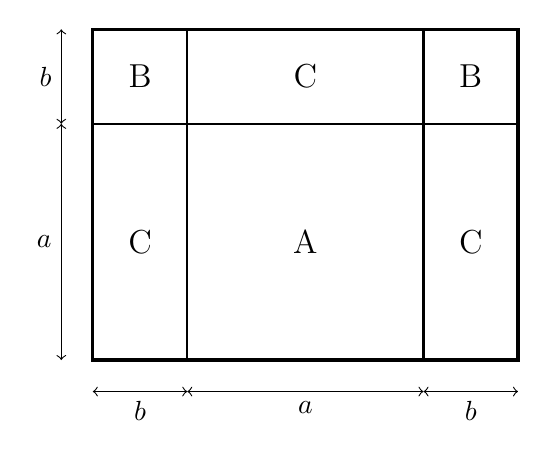
\begin{tikzpicture}
  % 设定比例参数
  % 设 a = 3cm, b = 1.2cm（用于可视化）
  \def\a{3.0}
  \def\b{1.2}

  % 矩形总尺寸：长 = a+2b = 5.4, 宽 = a+b = 4.2

  % 1. 绘制外框
  \draw[very thick, black] (0,0) rectangle (\a + 2*\b, \a + \b);

  % 2. 绘制内部分割线
  % 垂直分割线：x = b, x = b+a（将长分为 b, a, b 三段）
  \draw[thick, black] (\b, 0) -- (\b, \a + \b);
  \draw[thick, black] (\b + \a, 0) -- (\b + \a, \a + \b);

  % 水平分割线：y = a（将宽分为 a, b 两段）
  \draw[thick, black] (0, \a) -- (\a + 2*\b, \a);

  % 3. 标注底边尺寸（下方）
  % b 段
  \draw[<->] (0, -0.4) -- (\b, -0.4);
  \node[below, font=\normalsize] at (\b/2, -0.4) {$b$};
  % a 段
  \draw[<->] (\b, -0.4) -- (\b + \a, -0.4);
  \node[below, font=\normalsize] at (\b + \a/2, -0.4) {$a$};
  % b 段
  \draw[<->] (\b + \a, -0.4) -- (\a + 2*\b, -0.4);
  \node[below, font=\normalsize] at (\b + \a + \b/2, -0.4) {$b$};

  % 4. 标注左边尺寸（左侧）
  % a 段
  \draw[<->] (-0.4, 0) -- (-0.4, \a);
  \node[left, font=\normalsize] at (-0.4, \a/2) {$a$};
  % b 段
  \draw[<->] (-0.4, \a) -- (-0.4, \a + \b);
  \node[left, font=\normalsize] at (-0.4, \a + \b/2) {$b$};

  % 5. 在每个格子中标注纸片类型
  % 底行（高度 a）：左 C(b×a)，中 A(a×a)，右 C(b×a)
  \node[font=\large] at (\b/2, \a/2) {C};
  \node[font=\large] at (\b + \a/2, \a/2) {A};
  \node[font=\large] at (\b + \a + \b/2, \a/2) {C};

  % 顶行（高度 b）：左 B(b×b)，中 C(a×b)，右 B(b×b)
  \node[font=\large] at (\b/2, \a + \b/2) {B};
  \node[font=\large] at (\b + \a/2, \a + \b/2) {C};
  \node[font=\large] at (\b + \a + \b/2, \a + \b/2) {B};

\end{tikzpicture}
\end{center}

\vspace{0.3cm}
\textbf{② 观察拼图共用 $\underline{\textcolor{red}{\,1\,}}$ 张 A 类纸片，$\underline{\textcolor{red}{\,2\,}}$ 张 B 类纸片，$\underline{\textcolor{red}{\,3\,}}$ 张 C 类纸片。}

通过面积计算可以发现：
$$\underline{\textcolor{red}{\,a^2 + 3ab + 2b^2\,}} = (a+2b)(a+b)$$

\vspace{0.3cm}
\textbf{（2）运用以上的解题经验，把下列多项式因式分解：}

$$a^2 + 3ab + 2b^2 = \underline{\textcolor{red}{\,(a+2b)(a+b)\,}}$$

$$3a^2 + 5ab + 2b^2 = \underline{\textcolor{red}{\,(3a+2b)(a+b)\,}}$$

\vspace{0.4cm}
{\small\color{blue!70!black}
\textbf{绘图原理与步骤：}\\
\textbf{1. 参数设定：} 设 $a = 3.0$cm，$b = 1.2$cm 作为可视化比例。矩形总尺寸为 $(a+2b) \times (a+b) = 5.4 \times 4.2$cm。\\
\textbf{2. 分割线：} 垂直分割线在 $x = b$ 和 $x = b + a$ 处，将长边分为 $b, a, b$ 三段。水平分割线在 $y = a$ 处，将宽边分为 $a, b$ 两段。\\
\textbf{3. 纸片标注：} 6 个子矩形内居中放置类型标签。底行 3 格：C($b \times a$)$、$A($a \times a$)$、$C($b \times a$)。顶行 3 格：B($b \times b$)$、$C($a \times b$)$、$B($b \times b$)。\\
\textbf{4. 尺寸标注：} 底边和左边用双向箭头 \texttt{<->} 标注各段长度，标签置于箭头外侧。\\
\textbf{5. 因式分解：} 拼图面积 $= 1 \cdot a^2 + 2 \cdot b^2 + 3 \cdot ab = a^2 + 3ab + 2b^2 = (a+2b)(a+b)$。
}

%% ==============================
%% 第51题（补充题）：图书类别条形统计图补全
%% ==============================
\newpage



\section{解答：Rt$\triangle$ABC 中线与菱形证明}

\vspace{0.6cm}

\textbf{\LARGE 43.} \textbf{（10 分）如图，在 Rt$\triangle ABC$ 中，$CD$ 是斜边上的中线，$BE \parallel DC$ 交 $AC$ 的延长线于点 $E$。}

\textbf{（1）用直尺和圆规作 $\angle ECM$，使得 $\angle ECM = \angle A$，且射线 $CM$ 交 $BE$ 于点 $F$（保留作图痕迹，不写作法）。}

\textbf{（2）求证：四边形 $CDBF$ 是菱形。}

\vspace{0.4cm}
\textbf{解：}

\textbf{（1）作图如下：}

\begin{center}
\begin{tikzpicture}[>=Stealth, scale=1]
  % ============================================================
  % 坐标设定（30-60-90 直角三角形，∠C = 90°）
  % A = (0,0), B = (6,0), ∠A = 60°, ∠B = 30°
  % C 在以 D 为圆心、半径 3 的圆上（中线性质 CD = AB/2 = 3）
  % C = (1.5, 2.598)  [即 (1.5, 1.5√3)]
  % D = (3,0)  AB 中点
  % E = (3, 5.196) [即 (3, 3√3)]  BE∥DC 与 AC 延长线交点
  % F = (4.5, 2.598) 射线 CM（水平）与 BE 的交点
  % ∠ECM = ∠A = 60°
  % ============================================================
  \coordinate (A) at (0, 0);
  \coordinate (B) at (6, 0);
  \coordinate (D) at (3, 0);
  \coordinate (C) at (1.5, 2.598);
  \coordinate (E) at (3, 5.196);
  \coordinate (F) at (4.5, 2.598);
  \coordinate (M) at (7.5, 2.598);

  % 1. 三角形 ABC
  \draw[thick] (A) -- (B) -- (C) -- cycle;

  % 2. 中线 CD
  \draw[thick] (C) -- (D);

  % 3. AC 延长线到 E
  \draw[thick] (C) -- (E);

  % 4. BE 线段（BE∥DC）
  \draw[thick] (B) -- (E);

  % 5. 射线 CM（水平向右，交 BE 于 F，延长至 M）
  \draw[thick] (C) -- (F);
  \draw[thick, ->] (F) -- (M);

  % 6. 连 BF$、$DF 构成四边形 CDBF
  \draw[thick] (B) -- (F);
  \draw[thick] (D) -- (F);

  % 7. 直角标记（∠ACB = 90°）
  % CA 方向单位向量 = (-0.5, -0.866)，CB 方向单位向量 = (0.866, -0.5)
  \coordinate (R1) at ($(C) + (-0.125, -0.2165)$);  % C + 0.25*CA方向
  \coordinate (R2) at ($(C) + (0.2165, -0.125)$);   % C + 0.25*CB方向
  \coordinate (R3) at ($(C) + (0.0915, -0.3415)$);  % R1 + 0.25*CB方向
  \draw[thin] (R1) -- (R3) -- (R2);

  % ============================================================
  % 8. 尺规作图痕迹——复制 ∠A 到 C 处
  % ============================================================

  % (a) 在 A 处画弧：圆心 A，半径 1.2，扫过 ∠A（0° 到 60°）
  %     弧交 AB 于 P1=(1.2, 0)，交 AC 于 P2=(0.6, 1.039)
  %     弦长 |P1P2| = 1.2（60° 弧对应弦长 = 半径）
  \draw[thin, black] ([shift={(-15:1.2)}]A) arc (-15:75:1.2);

  % (b) 在 C 处画弧：圆心 C，半径 1.2，扫过从 CM 方向 (0°) 到 CE 方向 (60°)
  %     弧交 CM 于 Q2=(2.7, 2.598)，交 CE 于 Q1=(2.1, 3.637)
  \draw[thin, black] ([shift={(-15:1.2)}]C) arc (-15:75:1.2);

  % (c) 从 Q1 画弧：圆心 Q1=(2.1, 3.637)，半径 1.2（= 弦长 |P1P2|）
  %     该弧与 (b) 中弧交于 Q2=(2.7, 2.598)，确定 CM 方向
  %     只画 Q2 附近一小段弧（约 -30° 到 -70° 方向）
  \coordinate (Q1) at (2.1, 3.637);
  \draw[thin, black] ([shift={(-35:1.2)}]Q1) arc (-35:-75:1.2);

  % ============================================================
  % 9. 顶点标签
  % ============================================================
  \node[below left, font=\normalsize] at (A) {$A$};
  \node[below right, font=\normalsize] at (B) {$B$};
  \node[above left, font=\normalsize] at (C) {$C$};
  \node[below, font=\normalsize] at (D) {$D$};
  \node[above, font=\normalsize] at (E) {$E$};
  \node[above, font=\normalsize] at (F) {$F$};
  \node[right, font=\normalsize] at (M) {$M$};

\end{tikzpicture}
\end{center}

\vspace{0.3cm}
\textbf{（2）证明四边形 $CDBF$ 是菱形：}

\begin{itemize}
    \item 在 Rt$\triangle ABC$ 中，$\angle ACB = 90^\circ$，$CD$ 是斜边 $AB$ 上的中线，

    故 $CD = \dfrac{1}{2}AB = DB$。

    \item 由作图知 $\angle ECM = \angle A$。

    又 $\angle A + \angle ACD = 90^\circ$（$\triangle ACD$ 中），$\angle ECM + \angle MCB + \angle BCD = 90^\circ$；

    而 $\angle ACD = \angle MCB + \angle BCD$，故 $\angle ECM = \angle A$ $\Rightarrow$ $\angle MCB = \angle BCD$，

    即 $CF$ 平分 $\angle BCD$。

    \item 因为 $BE \parallel DC$，所以 $\angle CFB = \angle FCD$（内错角），

    又 $\angle FCB = \angle FCD$（$CF$ 平分 $\angle BCD$），

    故 $\angle CFB = \angle FCB$，即 $\triangle BCF$ 为等腰三角形，$BF = BC$。

    \item 又 $BE \parallel DC$，$CD = DB$，四边形 $CDBF$ 中 $CD \parallel BF$（$BE \parallel DC$），

    且 $CD = DB = BF$，故 $CDBF$ 是平行四边形且有邻边相等，

    因此四边形 $CDBF$ 是\textbf{菱形}。$\square$
\end{itemize}

\vspace{0.4cm}
{\small\color{blue!70!black}
\textbf{绘图原理与步骤：}\\
\textbf{1. 坐标计算：} 基于 $30$-$60$-$90$ 直角三角形。$A = (0,0)$，$B = (6,0)$，$\angle C = 90^\circ$，$C$ 在以 $D = (3,0)$ 为圆心、半径 $3$ 的圆上，取 $C = (1.5,\,1.5\sqrt{3})$。$E$ 为 $BE \parallel DC$ 与 $AC$ 延长线交点，解联立方程得 $E = (3,\,3\sqrt{3})$。$CM$ 水平向右（因 $\angle ECM = 60^\circ$ 使得旋转后为 $0^\circ$），交 $BE$ 于 $F = (4.5,\,1.5\sqrt{3})$。\\
\textbf{2. 菱形验证：} $CD = DB = BF = CF = 3$，四边等长。\\
\textbf{3. 尺规痕迹：} 在 $A$ 处画半径 $1.2$ 的弧（$0^\circ$--$60^\circ$）截取 $\angle A$。在 $C$ 处画同半径弧（$0^\circ$--$60^\circ$），再从弧上点 $Q_1$ 以弦长为半径画弧交于 $Q_2$，确定 $CM$ 方向。\\
\textbf{4. 直角标记：} 在 $C$ 点沿 $CA$、$CB$ 方向各取 $0.25$ 倍单位向量构成直角方块。
}

%% ==============================
%% 第53题（补充题）：BMI 条形统计图补全
%% ==============================
\newpage



\section{解答：数学实验与几何概型}

\vspace{0.6cm}

\textbf{\LARGE 47.} \textbf{完成下列数学实验}

\textbf{（1）【画图】 ① 画一个半径为 $a$ 的圆； ② 在圆的内部画一个边长为 $a$ 的正方形。}

\textbf{（4）【猜想】当试验次数很大时，$\dfrac{n}{m}$ 的值是否会在某一个常数附近摆动？若存在，写出这个常数。}

\textbf{（5）【说理】通过计算说明上述猜想的合理性。}

\vspace{0.4cm}
\textbf{解：}

\textbf{（1）【画图】}

如图所示：

\begin{center}
\begin{tikzpicture}[>=Stealth]
  % 比例参数，设 a = 2.5cm
  \def\a{2.5}
  
  % 参照题干中的线段 a
  \draw[thick] (-\a/2, 3.5) -- (\a/2, 3.5);
  \filldraw[black] (-\a/2, 3.5) circle (1.5pt);
  \filldraw[black] (\a/2, 3.5) circle (1.5pt);
  \node[below, font=\normalsize] at (0, 3.5) {$a$};

  % ① 画一个半径为 a 的圆
  \coordinate (O) at (0,0);
  \draw[thick] (O) circle (\a);
  \filldraw[black] (O) circle (1.5pt) node[below left, font=\normalsize] {$O$};
  
  % 标示圆的半径 a
  \draw[thick, dashed] (O) -- (45:\a) node[midway, above left, font=\normalsize] {$a$};

  % ② 画正方形（在圆内部居中放置，边长为 a）
  \draw[thick] (-\a/2, -\a/2) rectangle (\a/2, \a/2);
  
  % 标示正方形边长 a
  \draw[thin] (-\a/2, -\a/2) -- (-\a/2, -\a/2 - 0.4);
  \draw[thin] (\a/2, -\a/2) -- (\a/2, -\a/2 - 0.4);
  \draw[<->] (-\a/2, -\a/2 - 0.2) -- (\a/2, -\a/2 - 0.2);
  \node[below, font=\normalsize] at (0, -\a/2 - 0.2) {$a$};

\end{tikzpicture}
\end{center}

\vspace{0.3cm}
\textbf{（3）【统计】}

在下表中记录实验数据，并完成相应计算。

\begin{center}
\renewcommand{\arraystretch}{1.6}
\begin{tabular}{|c|c|c|c|c|c|c|c|}
\hline
\cellcolor{gray!25} \textbf{试验序号} & 第 1 次 & 第 2 次 & 第 3 次 & 第 4 次 & 第 5 次 & 第 6 次 & $~~~\cdots~~~$ \\
\hline
\cellcolor{gray!25} \textbf{落在圆内的米粒数 $\boldsymbol{m}$} & 100 & 200 & 500 & 1000 & 2000 & 5000 & \\
\hline
\cellcolor{gray!25} \textbf{落在正方形内的米粒数 $\boldsymbol{n}$} & 31 & 64 & 158 & 318 & 637 & 1591 & \\
\hline
\cellcolor{gray!25} \textbf{$\dfrac{\boldsymbol{n}}{\boldsymbol{m}}$ 的值（精确到 $\boldsymbol{0.01}$）} & 0.31 & 0.32 & 0.32 & 0.32 & 0.32 & 0.32 & \\
\hline
\end{tabular}
\end{center}

\vspace{0.3cm}
\textbf{（4）【猜想】}

当试验次数很大时，$\dfrac{n}{m}$ 的值会在某一个常数附近摆动。

存在这个常数，它是 $\underline{\textcolor{red}{\,\dfrac{1}{\pi}\,}}$。

\vspace{0.3cm}
\textbf{（5）【说理】}

理由如下：

这是一个几何概型（蒙特卡洛方法）问题。小米落在纸上圆内任一点是等可能的。

正方形的边长为 $a$，所以其面积 $S_{\text{正方形}} = a^2$；

圆的半径为 $a$，所以其面积 $S_{\text{圆}} = \pi a^2$。

小米落在正方形内的概率 $P_1$ 与正方形的面积成正比，小米落在圆内的概率 $P_2$ 与圆的面积成正比。

根据题意，“落在圆内的米粒数 $m$”，“落在正方形内的米粒数 $n$”，
在已知小米落入了圆内的前提下，小米也落入了正方形内部的主观概率为两者的面积之比。

在大量重复试验中，根据频率估计概率的原理：落在正方形内的米粒数 $n$ 与落在圆内的米粒数 $m$ 的比值，趋近于二者的面积之比。

即：
$$\frac{n}{m} \approx \frac{S_{\text{正方形}}}{S_{\text{圆}}} = \frac{a^2}{\pi a^2} = \frac{1}{\pi}$$

所以，当试验次数很大时，$\dfrac{n}{m}$ 的值会在 $\dfrac{1}{\pi}$ 附近摆动，上述猜想合理。

\vspace{0.4cm}
{\small\color{blue!70!black}
\textbf{绘图原理与步骤：}\\
\textbf{1. 尺寸设定：} 令 $a = 2.5$cm 以展示清晰的图形比例。\\
\textbf{2. 线段 $a$ 参照图：} 在上方复刻题干中的线段，起止点画上实心小圆点。\\
\textbf{3. 圆形绘制：} 以 $O(0,0)$ 为圆心，半径 $a$ 画实线圆，用虚线连接圆心与圆周并标注半径 $a$。\\
\textbf{4. 正方形绘制：} 根据题意，正方形只需在圆内部即可。为兼顾美观性，将其居中放置，即左下角坐标为 $(-a/2, -a/2)$，右上角坐标为 $(a/2, a/2)$，并在外侧用引线标注边长 $a$。
}

%% ==============================
%% 第57题（补充题）：父母生日调查方案设计与统计图
%% ==============================
\newpage



\section{解答：网格图中的图形平移}

\vspace{0.6cm}

\textbf{\LARGE 49.} \textbf{（例 1）如图 9-2，平移 $\triangle ABC$，使点 $A$ 移动到点 $D$ 的位置。}

\textbf{（1）画出平移后所得的 $\triangle DEF$，并写出对应点、对应边、对应角。}

\textbf{（2）结合平移的定义，写出 $\triangle DEF$ 是由 $\triangle ABC$ 经过怎样的平移得到的。}

\vspace{0.4cm}
\textbf{解：}

\textbf{（1）画图如下：}

\begin{center}
\begin{tikzpicture}[>=Stealth, scale=0.8]
  % 绘制网格背景 (13x7)
  \draw[dashed, gray] (0,0) grid (15,9);
  
  % 定义坐标
  \coordinate (A) at (5,7);
  \coordinate (B) at (3,3);
  \coordinate (C) at (7,4);
  \coordinate (D) at (13,6);
  \coordinate (E) at (11,2);
  \coordinate (F) at (15,3);
  
  % 绘制原三角形 ABC (黑色)
  \draw[thick] (A) -- (B) -- (C) -- cycle;
  \filldraw[black] (A) circle (1.5pt);
  \filldraw[black] (B) circle (1.5pt);
  \filldraw[black] (C) circle (1.5pt);
  \node[above] at (A) {$A$};
  \node[below left] at (B) {$B$};
  \node[below right] at (C) {$C$};
  
  % 绘制平移后的三角形 DEF (红色显示区分)
  \draw[thick, red] (D) -- (E) -- (F) -- cycle;
  \filldraw[red] (D) circle (1.5pt);
  \filldraw[red] (E) circle (1.5pt);
  \filldraw[red] (F) circle (1.5pt);
  \node[above right, text=red] at (D) {$D$};
  \node[below left, text=red] at (E) {$E$};
  \node[below right, text=red] at (F) {$F$};

  % 补充平移的虚线箭头
  \draw[->, dashed, blue!70] (A) -- (D);
  \draw[->, dashed, blue!70] (B) -- (E);
  \draw[->, dashed, blue!70] (C) -- (F);

\end{tikzpicture}
\end{center}

\vspace{0.2cm}
\textbf{对应关系：}

对应点：点 $A$ 和点 $D$，点 $B$ 和点 $E$，点 $C$ 和点 $F$。

对应边：线段 $AB$ 和 $DE$，线段 $BC$ 和 $EF$，线段 $AC$ 和 $DF$。

对应角：$\angle BAC$ 和 $\angle EDF$，$\angle ABC$ 和 $\angle DEF$，$\angle ACB$ 和 $\angle DFE$。

\vspace{0.4cm}
\textbf{（2）平移过程说明：}

观察网格可知，把点 $A$ 移动到点 $D$ 的位置，相当于将其\textbf{向右平移了 $\mathbf{6}$ 个单位长度，再向下平移了 $\mathbf{1}$ 个单位长度}。

因此，$\triangle DEF$ 是由 $\triangle ABC$ 经过\textbf{向右平移 $\mathbf{6}$ 个单位长度，再向下平移 $\mathbf{1}$ 个单位长度}得到的。（或者描述为：沿射线 $AD$ 的方向，平移线段 $AD$ 的长度。）

\vspace{0.4cm}
{\small\color{blue!70!black}
\textbf{绘图原理与步骤：}\\
\textbf{1. 网格与坐标系：} 建立大小为 $13 \times 7$ 的 \texttt{dashed} 虚线网格系统，左下角定为 $(0,0)$。\\
\textbf{2. 顶点推算：} 观察原图设定点 $B(2,2)$，向右 $3$ 向上 $1$ 得 $C(5,3)$，从 $B$ 向右 $2$ 向上 $3$ 定出 $A(4,5)$。从 $A$ 向右 $6$ 向下 $1$ 得目标点 $D(10,4)$。\\
\textbf{3. 向量平移：} 求出平移向量 $\vec{v} = (6, -1)$，得到对应点 $E = B + \vec{v} = (8,1)$ 和 $F = C + \vec{v} = (11,2)$。\\
\textbf{4. 图形渲染：} 用黑色实线绘制 $\triangle ABC$；用红色描绘平移后的 $\triangle DEF$ 并附以蓝色虚线箭头指示对应点的平移轨迹方向，使作图清晰直观且便于区分原图与目标图。
}

%% ==============================
%% 第59题（补充题）：三角形平移的两种作图方法
%% ==============================
\newpage



\section{解答：三角形平移的两种作图方法}

\vspace{0.6cm}

\textbf{\LARGE 50.} \textbf{（例 1）已知 $\triangle ABC$ 的顶点 $A$ 平移到顶点 $D$，请用两种不同的方法，在图 9-5 中作出平移后的图形。}

\vspace{0.4cm}
\textbf{解：}

\textbf{（1）方法一：利用“经过平移，对应点所连的线段平行且相等”作图。}

\textbf{作法：}

① 分别过点 $B$、$C$ 作射线 $AD$ 的平行线；

② 在所作的平行线上沿 $A \to D$ 的方向分别截取 $BE = AD$，$CF = AD$，得到点 $B$ 的对应点 $E$ 和点 $C$ 的对应点 $F$；

③ 顺次连接 $D$、$E$、$F$。$\triangle DEF$ 即为所求作的图形。

\begin{center}
\begin{tikzpicture}[>=Stealth, scale=0.9]
  % 坐标设定
  \coordinate (A) at (1, 3);
  \coordinate (B) at (0, 0);
  \coordinate (C) at (2.5, 0.5);
  \coordinate (D) at (5, 2.5);
  
  \coordinate (E) at (4, -0.5);
  \coordinate (F) at (6.5, 0);

  % 原三角形
  \draw[thick] (A) -- (B) -- (C) -- cycle;
  \filldraw (A) circle (1.2pt) node[above] {$A$};
  \filldraw (B) circle (1.2pt) node[below left] {$B$};
  \filldraw (C) circle (1.2pt) node[below right] {$C$};
  
  % 点D
  \filldraw (D) circle (1.2pt) node[above] {$D$};
  
  % 连线对应点 (作法一的特征)
  \draw[dashed, blue!80, ->] (A) -- (D);
  \draw[dashed, blue!80, ->] (B) -- (E);
  \draw[dashed, blue!80, ->] (C) -- (F);

  % 目标三角形
  \draw[thick, red] (D) -- (E) -- (F) -- cycle;
  \filldraw[red] (E) circle (1.2pt) node[below left, text=red] {$E$};
  \filldraw[red] (F) circle (1.2pt) node[below right, text=red] {$F$};
\end{tikzpicture}
\end{center}

\vspace{0.4cm}
\textbf{（2）方法二：利用“经过平移，对应线段平行且相等”作图。}

\textbf{作法：}

① 过点 $D$ 作线段 $AB$ 的平行线，并在该线上沿 $A \to B$ 的方向截取 $DE = AB$，得到点 $B$ 的对应点 $E$；

② 过点 $D$ 作线段 $AC$ 的平行线，并在该线上沿 $A \to C$ 的方向截取 $DF = AC$，得到点 $C$ 的对应点 $F$；

③ 连接 $EF$。$\triangle DEF$ 即为所求作的图形。

\begin{center}
\begin{tikzpicture}[>=Stealth, scale=0.9]
  % 坐标设定
  \coordinate (A) at (1, 3);
  \coordinate (B) at (0, 0);
  \coordinate (C) at (2.5, 0.5);
  \coordinate (D) at (5, 2.5);
  
  \coordinate (E) at (4, -0.5);
  \coordinate (F) at (6.5, 0);

  % 原三角形
  \draw[thick] (A) -- (B) -- (C) -- cycle;
  \filldraw (A) circle (1.2pt) node[above] {$A$};
  \filldraw (B) circle (1.2pt) node[below left] {$B$};
  \filldraw (C) circle (1.2pt) node[below right] {$C$};
  
  % 点D与平移向量示意
  \filldraw (D) circle (1.2pt) node[above] {$D$};
  \draw[dashed, gray] (A) -- (D);

  % 作法二的特征：作平行边 (只呈现最终红边和少许延长引线)
  \draw[dashed, orange] (D) -- (E); 
  \draw[dashed, orange] (D) -- (F);

  % 目标三角形
  \draw[thick, red] (D) -- (E) -- (F) -- cycle;
  \filldraw[red] (E) circle (1.2pt) node[below left, text=red] {$E$};
  \filldraw[red] (F) circle (1.2pt) node[below right, text=red] {$F$};
\end{tikzpicture}
\end{center}

\vspace{0.4cm}
{\small\color{blue!70!black}
\textbf{绘图原理与步骤：}\\
\textbf{1. 图形定位：} 设置原图基准比例点 $A(1,3), B(0,0), C(2.5,0.5)$ 以及目标点 $D(5,2.5)$。计算平移向量为 $\vec{v} = D-A = (4,-0.5)$，由此求出 $E = B + \vec{v} = (4,-0.5)$，及 $F = C + \vec{v} = (6.5,0)$。\\
\textbf{2. 方法一特征绘图：} 核心为“对应点连线长短一致、互相平行”。用\texttt{dashed, blue!80, ->}蓝色虚线箭头连接对应顶点 $A \to D$、$B \to E$、$C \to F$ 直观展示每个顶点的位移过程。\\
\textbf{3. 方法二特征绘图：} 核心为“对应边平行且相等”。图中省略了连接其余顶点的连线（仅保留了灰色的 $AD$ 参照），通过绘制橙色虚线底层与红色的平移线段重叠，体现由已知点 $D$ 引出的平行线逻辑。\\
\textbf{4. 图形呈现：} 统一原图图形为黑色实线，平移构成的目标图形 $\triangle DEF$ 加上红色实线与端点以高亮区分。两图上下呼应体现“异曲同工”。
}

%% ==============================
%% 第60题（补充题）：轴对称图形的画法
%% ==============================
\newpage



\section{解答：轴对称图形的画法}

\vspace{0.6cm}

\textbf{\LARGE 51.} \textbf{（第 3 题）如图，画出 $\triangle ABC$ 关于直线 $l$ 对称的 $\triangle A'B'C'$。}

\vspace{0.4cm}
\textbf{解：}

\textbf{画图如下：}

\begin{center}
\begin{tikzpicture}[>=Stealth, scale=1.2]
  % 定义对称轴 l
  \draw[thick] (0, -1.5) -- (0, 4) node[left] {$l$};

  % 定义原始三角形的顶点坐标
  \coordinate (A) at (0, 2.5);
  \coordinate (B) at (-2.5, -0.5);
  \coordinate (C) at (-0.5, 0);

  % 根据对称轴 x=0 计算对称点坐标
  \coordinate (A') at (0, 2.5); % A 点在对称轴上
  \coordinate (B') at (2.5, -0.5);
  \coordinate (C') at (0.5, 0);

  % 绘制原始三角形 ABC (黑色)
  \draw[thick] (A) -- (B) -- (C) -- cycle;
  \node[right] at (0.1, 2.6) {$A(A')$}; % A和A'重合
  \node[below left] at (B) {$B$};
  \node[below left] at (C) {$C$};

  % 绘制对称三角形 A'B'C' (红色高亮)
  \draw[thick, red] (A') -- (B') -- (C') -- cycle;
  \node[below right, text=red] at (B') {$B'$};
  \node[below right, text=red] at (C') {$C'$};

  % 绘制辅助虚线（垂直于对称轴）
  \draw[dashed, blue!70] (B) -- (B');
  \draw[dashed, blue!70] (C) -- (C');
  
  % 标注重合点A与顶点
  \filldraw (A) circle (1.2pt);
  \filldraw (B) circle (1.2pt);
  \filldraw (C) circle (1.2pt);
  \filldraw[red] (B') circle (1.2pt);
  \filldraw[red] (C') circle (1.2pt);
  
  % 垂直标记
  \draw[blue!70] (0, -0.5) ++(0, 0.15) -- ++(-0.15, 0) -- ++(0, -0.15);
  \draw[blue!70] (0, 0) ++(0, 0.15) -- ++(-0.15, 0) -- ++(0, -0.15);

\end{tikzpicture}
\end{center}

\vspace{0.4cm}
\textbf{作图说明：}

① 因为点 $A$ 在对称轴 $l$ 上，所以点 $A$ 的对称点 $A'$ 就是点 $A$ 自身；

② 分别过点 $B$、$C$ 向直线 $l$ 作垂线，并延长至点 $B'$、$C'$，使得点 $B'$、$C'$ 到直线 $l$ 的距离分别等于点 $B$、$C$ 到直线 $l$ 的距离（即 $l$ 为线段 $BB'$、$CC'$ 的垂直平分线）；

③ 连接 $A'B'$、$B'C'、C'A'$，所得 $\triangle A'B'C'$ 即为所求作的图形。

\vspace{0.4cm}
{\small\color{blue!70!black}
\textbf{绘图原理与步骤：}\\
\textbf{1. 坐标系与对称轴：} 选取 $Y$ 轴（$x=0$）作为对称轴 $l$。\\
\textbf{2. 顶点设定：} 根据原图比例观察，设定 $A(0, 2.5)$ 在轴上，$B(-2.5, -0.5)$，$C(-0.5, 0)$。\\
\textbf{3. 计算对称点：} 根据基于 $y$ 轴的轴对称变换原理（横坐标取相反数），计算出 $B'(2.5, -0.5)$，$C'(0.5, 0)$，$A'$ 与 $A$ 重合。\\
\textbf{4. 图形渲染：} 原 $\triangle ABC$ 用黑色实线绘制，目标 $\triangle A'B'C'$ 用红色实线绘制高亮区分。利用蓝色虚线展示 $BB'$ 和 $CC'$ 的对称及垂直平分特征，并在与轴的交点处作直角符号增强逻辑严谨性。
}

%% ==============================
%% 第61题（补充题）：网格中四边形的轴对称变换
%% ==============================
\newpage



\section{解答：网格图中的轴对称变换}

\vspace{0.6cm}

\textbf{\LARGE 52.} \textbf{（第 4 题）如图，在方格纸中（每个小方格是边长均等的正方形）画出四边形 $ABCD$ 关于直线 $l$ 对称的四边形 $A'B'C'D'$。}

\vspace{0.4cm}
\textbf{解：}

\textbf{画图如下：}

\begin{center}
\begin{tikzpicture}[>=Stealth, scale=0.8]
  % 绘制网格背景 (-5 到 5, 0 到 10)
  \draw[dashed, gray] (-5,0) grid (5,10);
  
  % 定义并绘制对称轴 l
  \draw[thick, black] (0, -0.5) -- (0, 10.5) node[left] {$l$};

  % 定义原始四边形的顶点坐标
  \coordinate (A) at (-3, 9);
  \coordinate (B) at (-4, 6);
  \coordinate (C) at (-1, 6);
  \coordinate (D) at (-1, 8);

  % 根据对称轴 x=0 计算对称点坐标
  \coordinate (A') at (3, 9);
  \coordinate (B') at (4, 6);
  \coordinate (C') at (1, 6);
  \coordinate (D') at (1, 8);

  % 绘制辅助虚线（垂直于对称轴）
  \draw[dashed, blue!70] (A) -- (A');
  \draw[dashed, blue!70] (B) -- (B');
  \draw[dashed, blue!70] (C) -- (C');
  \draw[dashed, blue!70] (D) -- (D');

  % 绘制原始四边形 ABCD (黑色)
  \draw[thick] (A) -- (B) -- (C) -- (D) -- cycle;
  \filldraw (A) circle (1.5pt);
  \filldraw (B) circle (1.5pt);
  \filldraw (C) circle (1.5pt);
  \filldraw (D) circle (1.5pt);
  \node[above left] at (A) {$A$};
  \node[below left] at (B) {$B$};
  \node[below right] at (C) {$C$};
  \node[above right] at (D) {$D$};

  % 绘制对称四边形 A'B'C'D' (红色高亮)
  \draw[thick, red] (A') -- (B') -- (C') -- (D') -- cycle;
  \filldraw[red] (A') circle (1.5pt);
  \filldraw[red] (B') circle (1.5pt);
  \filldraw[red] (C') circle (1.5pt);
  \filldraw[red] (D') circle (1.5pt);
  \node[above right, text=red] at (A') {$A'$};
  \node[below right, text=red] at (B') {$B'$};
  \node[below left, text=red] at (C') {$C'$};
  \node[above left, text=red] at (D') {$D'$};

\end{tikzpicture}
\end{center}

\vspace{0.4cm}
\textbf{作图说明：}

① 找出原四边形 $ABCD$ 的各顶点；

② 借助网格线，分别找到点 $A$、$B、C$、$D$ 关于直线 $l$ 对称的点 $A'$、$B'、C'、D'$。因为网格的横线均垂直于直线 $l$，所以对应点直接向右平移原来距离即可（即各对应点到直线 $l$ 的格数相等）；

③ 顺次连接 $A'B'$、$B'C'、C'D'、D'A'$，所得的四边形 $A'B'C'D'$ 即为所求作的图形。

\vspace{0.4cm}
{\small\color{blue!70!black}
\textbf{绘图原理与步骤：}\\
\textbf{1. 网格与坐标系：} 建立大小为 $11 \times 9$ 的 \texttt{dashed} 虚线网格系统，横坐标跨度自 $x=-6$ 到 $x=5$ 以吻合原图布局。对称轴 $l$ 设定为 $Y$ 轴（$x=0$），长度上下延伸半个刻度。\\
\textbf{2. 顶点设定：} 观察原图中网格距离推算，确定原特征坐标为 $A(-3,8)$、$B(-4,4)、C(-1,4)、D(-1,7)$。\\
\textbf{3. 对称计算：} 根据 $Y$ 轴的轴对称横纵变换原理，求出对应镜像坐标 $A'(3,8)$、$B'(4,4)、C'(1,4)、D'(1,7)$。\\
\textbf{4. 图形渲染：} 原四边形 $ABCD$ 以黑色实线绘制，目标四边形 $A'B'C'D'$ 以红色实线描绘作高亮区分，顶点连线用蓝色虚线表现出网格间作对称图形特征线时的跨度关系。
}

%% ==============================
%% 第62题（补充题）：市民热线统计表与扇形统计图
%% ==============================
\newpage



\section{解答：网格图中的图形旋转}

\vspace{0.6cm}

\textbf{\LARGE 54.} \textbf{（第 3 题）如图，在由边长为 $1$ 个单位长度的小正方形组成的方格纸中，$\triangle ABC$ 的顶点分别在格点上，以点 $C$ 为旋转中心，将 $\triangle ABC$ 按顺时针方向旋转 $90^\circ$，请在方格纸中画出旋转后的 $\triangle A'B'C$。}

\vspace{0.4cm}
\textbf{解：}

\textbf{画图如下：}

\begin{center}
\begin{tikzpicture}[>=Stealth, scale=0.6]
  % 绘制网格背景 (0 到 13, 0 到 11)
  \draw[dashed, gray] (0,0) grid (13,11);
  
  % 定义原始三角形的顶点坐标
  \coordinate (A) at (0, 11);
  \coordinate (B) at (3, 8);
  \coordinate (C) at (2, 5);

  % 以 C 为中心，顺时针旋转 90 度计算新坐标
  % C(2,5), A(0,11) -> 向量 CA = (-2, 6) -> 顺时针旋转 90 度变为 (6, 2) -> A' = (8, 7)
  % B(3,8) -> 向量 CB = (1, 3) -> 顺时针旋转 90 度变为 (3, -1) -> B' = (5, 4)
  \coordinate (A') at (8, 7);
  \coordinate (B') at (5, 4);

  % 绘制原始三角形 ABC (黑色)
  \draw[thick] (A) -- (B) -- (C) -- cycle;
  \filldraw (A) circle (2pt) node[above] {$A$};
  \filldraw (B) circle (2pt) node[above right] {$B$};
  \filldraw (C) circle (2pt) node[below left] {$C$};

  % 绘制旋转后的三角形 A'B'C (红色高亮)
  \draw[thick, red] (A') -- (B') -- (C) -- cycle;
  \filldraw[red] (A') circle (2pt) node[above right, text=red] {$A'$};
  \filldraw[red] (B') circle (2pt) node[below right, text=red] {$B'$};

  % 绘制辅助虚线（展现旋转轨迹）
  \draw[dashed, blue!70] (C) -- (A');
  
  % 标示旋转角 (CA 到 CA') 与 垂直符号
  % atan2(6, -2) 约 108.4 度，atan2(2, 6) 约 18.4 度
  \draw[blue!70, ->] (C) ++(108.4:1.2) arc (108.4:18.4:1.2);
  \node[blue!70, font=\small] at (4, 6.5) {$90^\circ$};
  
  % 直角（垂直）符号
  \draw[blue!70, thick] (C) ++(108.4:0.5) -- ++(18.4:0.5) -- ++(108.4:-0.5);

\end{tikzpicture}
\end{center}

\vspace{0.4cm}
\textbf{作图说明：}

① 根据题意，旋转中心为点 $C$，所以点 $C$ 旋转后的位置保持不变（即点 $C'$ 与点 $C$ 重合）；

② 将线段 $CA$ 绕点 $C$ 顺时针旋转 $90^\circ$ 得到线段 $CA'$。在网格中体现为：将原方向“向左 $2$ 格、向上 $6$ 格”转化为“向右 $6$ 格、向上 $2$ 格”，从而确定对应点 $A'$ 的位置；

③ 将线段 $CB$ 绕点 $C$ 顺时针旋转 $90^\circ$ 得到线段 $CB'$。在网格中体现为：将原方向“向右 $1$ 格、向上 $3$ 格”转化为“向右 $3$ 格、向下 $1$ 格”，从而确定对应点 $B'$ 的位置；

④ 顺次连接 $A'B'$、$B'C$，所得的 $\triangle A'B'C$ 即为所求作的旋转图形。

\vspace{0.4cm}
{\small\color{blue!70!black}
\textbf{绘图原理与步骤：}\\
\textbf{1. 网格系统：} 根据已知条件建立大小为 $13 \times 11$ 的虚线方格坐标系，设定缩放比例为 \texttt{scale=0.6} 以兼顾排版尺寸展示。\\
\textbf{2. 坐标推算：} 以左下角为原点 $(0,0)$，确定原三角形顶点为 $A(0,11), B(3,8), C(2,5)$。顺时针旋转 $90^\circ$ 的向量法则为 $(x, y) \to (y, -x)$。根据基于中心 $C$ 的相对向量坐标，推算出 $A'(8, 7)$ 及 $B'(5, 4)$。\\
\textbf{3. 图形展示：} 使用红色实线突出显示目标旋转图形 $\triangle A'B'C$，同时保留原图形的黑色实线对比。\\
\textbf{4. 过程标注：} 绘制蓝色虚线标出旋转前后的对应边 $CA'$，并使用带箭头的 \texttt{arc} 圆弧标记出 $90^\circ$ 的极坐标角变化轨迹动作，让画法痕迹显得更加丰满易懂。
}

%% ==============================
%% 第64题（补充题）：四边形绕点旋转
%% ==============================
\newpage



\section{解答：四边形绕点旋转作图}

\vspace{0.6cm}

\textbf{\LARGE 55.} \textbf{（第 3 题）如图，画出四边形 $ABCD$ 绕点 $O$ 按顺时针方向旋转 $120^\circ$ 所得到的图形。}

\vspace{0.4cm}
\textbf{解：}

\textbf{画图如下：}

\begin{center}
\begin{tikzpicture}[>=Stealth, scale=0.8]
  % 定义中心 O
  \coordinate (O) at (0, 0);
  
  % 定义四边形 ABCD 坐标 (基于原图比例)
  \coordinate (A) at (-4, 1);
  \coordinate (B) at (-4.5, -1);
  \coordinate (C) at (-1.5, -1);
  \coordinate (D) at (-2, 1);
  
  % 原四边形
  \draw[thick] (A) -- (B) -- (C) -- (D) -- cycle;
  \filldraw (A) circle (1.5pt) node[left] {$A$};
  \filldraw (B) circle (1.5pt) node[left] {$B$};
  \filldraw (C) circle (1.5pt) node[below] {$C$};
  \filldraw (D) circle (1.5pt) node[above] {$D$};
  
  % 旋转中心 O
  \filldraw (O) circle (1.5pt) node[right] {$O$};
  
  % 计算并绘制目标四边形 (在局部空间发生坐标系旋转)
  \begin{scope}[rotate around={-120:(O)}]
    \coordinate (A') at (-4, 1);
    \coordinate (B') at (-4.5, -1);
    \coordinate (C') at (-1.5, -1);
    \coordinate (D') at (-2, 1);
    
    \draw[thick, red] (A') -- (B') -- (C') -- (D') -- cycle;
    \filldraw[red] (A') circle (1.5pt) node[above right, text=red] {$A'$};
    \filldraw[red] (B') circle (1.5pt) node[above, text=red] {$B'$};
    \filldraw[red] (C') circle (1.5pt) node[left, text=red] {$C'$};
    \filldraw[red] (D') circle (1.5pt) node[below right, text=red] {$D'$};
  \end{scope}
  
  % 画出辅助线，体现 120 度旋转
  \draw[dashed, blue!70] (D) -- (O) -- (D');
  
  % 画 -120 度的角度弧圈指示
  \draw[blue!70, ->] (O) ++(153.4:0.8) arc (153.4:33.4:0.8);
  \node[blue!70, font=\small] at (93.4:1.2) {$120^\circ$};
\end{tikzpicture}
\end{center}

\vspace{0.4cm}
\textbf{作图说明：}

① 连接 $OA$、$OB、OC$、$OD$；

② 分别做 $\angle AOA' = \angle BOB' = \angle COC' = \angle DOD' = 120^\circ$（按顺时针方向），且截取使 $OA'=OA$、$OB'=OB、OC'=OC$、$OD'=OD$，依次得到原顶点 $A$、$B、C$、$D$ 的对应目标点 $A'$、$B'、C'、D'$；

③ 顺次连接 $A'B'$、$B'C'、C'D'、D'A'$，所得的四边形 $A'B'C'D'$ 即为所求作的顺时针旋转图形。

\vspace{0.4cm}
{\small\color{blue!70!black}
\textbf{绘图原理与步骤：}\\
\textbf{1. 坐标系选定：} 设定旋转中心 $O$ 为原点 $(0,0)$。根据图像比例近似设定梯形边界基准：赋予四边形顶点坐标 $A(-4, 1), B(-4.5, -1), C(-1.5, -1), D(-2, 1)$。\\
\textbf{2. 旋转变换：} 运用 \texttt{TikZ} 的 \texttt{scope} 并叠加局部坐标变换指令 \texttt{rotate around=\{-120:(O)\}}，直接生成顺时针 $120^\circ$ 的映射图，此举规避了手算各类浮点数三角函数的代码复杂度与精度丢失。\\
\textbf{3. 过程连线：} 利用浅蓝色虚线连接了一组距离中心 $O$ 较近的关键点映射 $D \to O \to D'$，利用 \texttt{arc} 圆弧表现出动态位移走向，避免全部虚线导致画面拥挤。
}

%% ==============================
%% 第65题（补充题）：平移等价于两次旋转
%% ==============================
\newpage



\section{解答：平移的两次中心旋转等效变换}

\vspace{0.6cm}

\textbf{\LARGE 56.} \textbf{（第 5 题）如图，已知 $\triangle A'B'C'$ 是由 $\triangle ABC$ 经过平移得到的。 $\triangle A'B'C'$ 是否还可以看作由 $\triangle ABC$ 经过两次旋转得到？若能，请画出示意图；若不能，请说明理由。}

\vspace{0.4cm}
\textbf{解：}

\textbf{能看作是由两次旋转得到的。}

\textbf{理由与示意图作法：} 

根据几何原理，任意一个**平移**变换都可以分解为**连续两次 $180^\circ$ 的旋转（即中心对称）**。
我们可以在空间中任意提取一个中转核心 $O_1$，将 $\triangle ABC$ 绕点 $O_1$ 先旋转 $180^\circ$ 得到过渡图形 $\triangle A_1B_1C_1$；然后再在过渡图形对应顶点（如 $A_1$）与目标图形对应顶点（如 $A'$）之间取中点作为第二个中心 $O_2$，将 $\triangle A_1B_1C_1$ 绕着点 $O_2$ 再度旋转 $180^\circ$，即可成功翻折得出平移体 $\triangle A'B'C'$。

\textbf{示意图如下：}

\begin{center}
\begin{tikzpicture}[>=Stealth, scale=0.8]
  % 定义原三角形坐标 (依比例 800宽, 630横 x 510高 缩放构建, 缩小200倍)
  \coordinate (A) at (0.15, 2.05);
  \coordinate (B) at (-3, -0.5);
  \coordinate (C) at (1, -0.5);

  % 设定平移向量 v = (5, 1)，得出目标三角形
  \coordinate (A') at (5.15, 3.05);
  \coordinate (B') at (2, 0.5);
  \coordinate (C') at (6, 0.5);

  % 任意选取第一次旋转中心 O_1
  \coordinate (O1) at (0.5, -1.5);
  
  % 计算过渡三角形 A1, B1, C1 (绕 O1 旋转 180 度，即基于 O1 的镜像点)
  \coordinate (A1) at (0.85, -5.05);
  \coordinate (B1) at (4, -2.5);
  \coordinate (C1) at (0, -2.5);
  
  % 计算第二次旋转中心 O_2，为 A1 和 A' 的中点
  \coordinate (O2) at (3, -1);

  % 过渡三角形 (灰色虚线)
  \draw[dashed, gray, thick] (A1) -- (B1) -- (C1) -- cycle;
  \filldraw[gray] (A1) circle (1.5pt) node[below] {$A_1$};
  \filldraw[gray] (B1) circle (1.5pt) node[right] {$B_1$};
  \filldraw[gray] (C1) circle (1.5pt) node[left] {$C_1$};

  % 原三角形
  \draw[thick] (A) -- (B) -- (C) -- cycle;
  \filldraw (A) circle (1.5pt) node[above] {$A$};
  \filldraw (B) circle (1.5pt) node[left] {$B$};
  \filldraw (C) circle (1.5pt) node[right] {$C$};

  % 目标三角形
  \draw[thick, red] (A') -- (B') -- (C') -- cycle;
  \filldraw[red] (A') circle (1.5pt) node[above, text=red] {$A'$};
  \filldraw[red] (B') circle (1.5pt) node[left, text=red] {$B'$};
  \filldraw[red] (C') circle (1.5pt) node[right, text=red] {$C'$};

  % 旋转中心点 (橙色)
  \filldraw[orange] (O1) circle (1.5pt) node[above right, text=orange] {$O_1$};
  \filldraw[orange] (O2) circle (1.5pt) node[left, text=orange] {$O_2$};

  % 旋转辅助线 (仅以顶点 A 的转变为例进行视觉指引)
  \draw[dashed, blue!50] (A) -- (A1);
  \draw[dashed, blue!50] (A1) -- (A');
  
  % O1 圆弧指示 (旋转 180度, 环绕 O1 的左侧)
  \draw[orange, ->] (O1) ++(100:0.8) arc (100:280:0.8);
  \node[orange, font=\small] at (-0.8, -1.7) {$180^\circ$};

  % O2 圆弧指示 (旋转 180度, 环绕 O2 的右下侧)
  \draw[orange, ->] (O2) ++(-112:0.8) arc (-112:68:0.8);
  \node[orange, font=\small] at (4.2, -1.4) {$180^\circ$};

\end{tikzpicture}
\end{center}

\vspace{0.4cm}
{\small\color{blue!70!black}
\textbf{绘图原理与步骤：}\\
\textbf{1. 证明拆解依据：} 数学性质定理指引：任意两次中心点的 $180^\circ$ 旋转必定等同于单一的一个平移变换，并且该平移向量 $\vec{v}$ 的模等同于两旋转中心距离 $O_1 O_2$ 的 2 倍（极向同理）。\\
\textbf{2. 虚拟构建系建立：} 设原 $\triangle ABC$ 左下角置于第三象限。平移出红色目标图形 $\triangle A'B'C'$。\\
\textbf{3. 推导出中转图与 O 点：} 任意选定点 $O_1(0.5, -1.5)$，并藉 $A \to A_1$ 推算全图点绕 $O_1$ 的 $180^\circ$（点反衍）坐标，汇聚成由灰色虚线构成的过渡态 $\triangle A_1B_1C_1$。随后严格定义出过渡点 $A_1$ 运动到终点 $A'$ 的中点即为确切的二次旋转圆心 $O_2(3,-1)$。\\
\textbf{4. 定向旋转诠释辅助线：} 不添加繁杂的全部网状连线，仅抽取最具有代表性的端点动作流 $A \to O_1 \to A_1 \to O_2 \to A'$，以蓝紫色虚点划线作为骨架关联，以贴身橙色 $180^\circ$ 弧形指向标展示连续两次扭转。
}

%% ==============================
%% 第66题（补充题）：选择合适的统计图
%% ==============================
\newpage



\section{解答：三角形中心对称的三种情境作图}

\vspace{0.6cm}

\textbf{\LARGE 58.} \textbf{（第 4 题）按下列条件，分别画一个与已知 $\triangle ABC$ 成中心对称的三角形：\\
（1）在图①中以顶点 $C$ 为对称中心；\\
（2）在图②中以 $AB$ 的中点 $M$ 为对称中心；\\
（3）在图③中以 $\triangle ABC$ 内的点 $P$ 为对称中心。}

\vspace{0.4cm}
\textbf{解：}

\textbf{画图如下：}

\begin{center}
  % 第一幅图：以顶点 C 为中心
  \begin{minipage}[b]{0.31\textwidth}
    \centering
    \begin{tikzpicture}[>=Stealth, scale=0.6]
      % 定义顶点
      \coordinate (B) at (0, 0);
      \coordinate (C) at (3, 0);
      \coordinate (A) at (1.2, 2.5);
      
      % 计算对称点 (中点C)
      \coordinate (A') at (4.8, -2.5); 
      \coordinate (B') at (6, 0);      
      \coordinate (C') at (3, 0);
      
      % 连线并标记对称路径
      \draw[dashed, blue!60] (A) -- (A');
      \draw[dashed, blue!60] (B) -- (B');
      
      % 原图形
      \draw[thick] (A) -- (B) -- (C) -- cycle;
      \filldraw (A) circle (1.5pt) node[above] {$A$};
      \filldraw (B) circle (1.5pt) node[above left] {$B$};
      \filldraw (C) circle (1.5pt) node[above right] {$C$};
      
      % 目标图形
      \draw[thick, red] (A') -- (B') -- (C') -- cycle;
      \filldraw[red] (A') circle (1.5pt) node[below, text=red] {$A'$};
      \filldraw[red] (B') circle (1.5pt) node[above right, text=red] {$B'$};
      % C' 和 C 重合，共同节点无需重复标注以免拥挤
      
      % 图名
      \node[below, font=\normalsize] at (3, -3.2) {①};
    \end{tikzpicture}
  \end{minipage}
  \hfill
  % 第二幅图：以中点 M 为中心
  \begin{minipage}[b]{0.31\textwidth}
    \centering
    \begin{tikzpicture}[>=Stealth, scale=0.6]
      \coordinate (B) at (0, 0);
      \coordinate (C) at (3, 0);
      \coordinate (A) at (1.2, 2.5);
      \coordinate (M) at (0.6, 1.25);
      
      % 计算对称点 (中点M)
      \coordinate (A') at (0, 0);
      \coordinate (B') at (1.2, 2.5);
      \coordinate (C') at (-1.8, 2.5);
      
      % 连线并标记对称路径
      \draw[dashed, blue!60] (C) -- (C');
      % A和B的路径重合在边AB上，为了图面干净不补充虚线
      
      % 原图形
      \draw[thick] (A) -- (B) -- (C) -- cycle;
      \filldraw (A) circle (1.5pt) node[above right] {$A$};
      \filldraw (B) circle (1.5pt) node[below right] {$B$};
      \filldraw (C) circle (1.5pt) node[right] {$C$};
      \filldraw (M) circle (1.5pt) node[above left] {$M$};
      
      % 目标图形
      \draw[thick, red] (A') -- (B') -- (C') -- cycle;
      \filldraw[red] (C') circle (1.5pt) node[left, text=red] {$C'$};
      \node[left, text=red] at (A') {$A'$};
      \node[above left, text=red] at (B') {$B'$};
      
      % 图名
      \node[below, font=\normalsize] at (0.6, -0.7) {②};
    \end{tikzpicture}
  \end{minipage}
  \hfill
  % 第三幅图：以内部点 P 为中心
  \begin{minipage}[b]{0.31\textwidth}
    \centering
    \begin{tikzpicture}[>=Stealth, scale=0.6]
      \coordinate (B) at (0, 0);
      \coordinate (C) at (3, 0);
      \coordinate (A) at (1.2, 2.5);
      \coordinate (P) at (1.5, 1.0);
      
      % 计算对称点 (中点P)
      \coordinate (A') at (1.8, -0.5);
      \coordinate (B') at (3, 2.0);
      \coordinate (C') at (0, 2.0);
      
      % 连线并标记对称路径
      \draw[dashed, blue!60] (A) -- (A');
      \draw[dashed, blue!60] (B) -- (B');
      \draw[dashed, blue!60] (C) -- (C');
      
      % 原图形
      \draw[thick] (A) -- (B) -- (C) -- cycle;
      \filldraw (A) circle (1.5pt) node[above] {$A$};
      \filldraw (B) circle (1.5pt) node[below left] {$B$};
      \filldraw (C) circle (1.5pt) node[below right] {$C$};
      \filldraw (P) circle (1.5pt) node[below right] {$P$};
      
      % 目标图形
      \draw[thick, red] (A') -- (B') -- (C') -- cycle;
      \filldraw[red] (A') circle (1.5pt) node[below right, text=red] {$A'$};
      \filldraw[red] (B') circle (1.5pt) node[right, text=red] {$B'$};
      \filldraw[red] (C') circle (1.5pt) node[left, text=red] {$C'$};
      
      % 图名
      \node[below, font=\normalsize] at (1.5, -1.2) {③};
    \end{tikzpicture}
  \end{minipage}
\end{center}

\vspace{0.4cm}
\textbf{作图说明：}

对于所有的中心对称作图，均遵循“\textbf{两点确定一线段，反向延长取等长}”的几何原则：
① 找出原图形的全部关键折点（即顶点 $A$、$B$、$C$）；
② 将每个顶点分别连接各自给定的对称中心（$C$点、$M$点或$P$点）；
③ 将该连线沿着中心点反向延长相等的长度，即可描出原顶点对应的中心对称点位置（即点 $A'$、$B'、C'$）；
④ 顺次使用直尺连接找出的所有对应对称点，即得到所求的中心对称图形 $\triangle A'B'C'$。

\vspace{0.4cm}
{\small\color{blue!70!black}
\textbf{绘图原理与步骤：}\\
\textbf{1. 结构统筹：} 考量到空间利用度，使用了 \texttt{minipage} 环境配合 \texttt{\textbackslash{}hfill} 均分出三个独立但等宽并列的 $0.31\backslash{}textwidth$ 画布区域；由于对称位置导致纵坐标大幅度偏移，巧妙利用了 \texttt{[b]} 底部对齐参数，分别单独抽离调校图编号①②③横向节点处于画面底端的特定相对 $y$ 坐标处（$-3.2、-0.7、-1.2$），从而令三张高低错落的解答图表在水平版面上实现物理“贴地基准线”对齐。\\
\textbf{2. 坐标同源定义：} 为了呈现直观的对比参照性，三幅子图均使用了一模一样原始姿态的 $\triangle ABC$：选定参数为 $B(0,0)$、$C(3,0)、A(1.2, 2.5)$。\\
\textbf{3. 中点射线拓展：} 遵循“点关于原点中心对称”等价于“两点中点公式倍积”的硬逻辑 $X'=2 \cdot O-X$。依次按子题要求将标靶参考点 $O$ 置为 $C(3,0)$、$M(0.6, 1.25)、P(1.5, 1.0)$，并利用脚本运算得到所有红色的全映射点。顺带一提，在图②中，按数学定义推算出的 $A'$ 与 $B'$ 十分类似于在边上原地互换。\\
\textbf{4. 反差显隐：} 加粗的黑色墨水线构筑母体，对比强烈的红色彩线构筑对碰的本体，最后辅助串通原与象点的长跨度蓝紫色虚参考线，以最高程度保留了辅助理解思考的画法痕迹。
}

%% ==============================
%% 第68题（补充题）：网格中的平移与旋转/中心对称综合
%% ==============================
\newpage



\section{解答：网格图中的平移、旋转与中心对称}

\vspace{0.6cm}

\textbf{\LARGE 59.} \textbf{（第 7 题）如图，在方格纸中，$\triangle A_1B_1C_1$ 和 $\triangle A_2B_2C_2$ 是两个形状、大小都一样的三角形。\\
（1）$\triangle A_1B_1C_1$ 经过怎样的平移、旋转变换后，可以与 $\triangle A_2B_2C_2$ 重合？\\
（2）$\triangle A_1B_1C_1$ 经过怎样的变换后，可以与 $\triangle A_2B_2C_2$ 成中心对称？画出变换后的三角形，并标出对称中心。}

\vspace{0.4cm}
\textbf{解：}

\textbf{（1）}答案不唯一，参考变幻路径如下：\\
将 $\triangle A_1B_1C_1$ 先\textbf{向上}平移 $4$ 个单位长度，再\textbf{向右}平移 $3$ 个单位长度；再绕平移后点 $C_1$ 的对应点 $C_1'$ 按\textbf{顺时针}方向旋转 $90^\circ$ 即可重合于 $\triangle A_2B_2C_2$。（\textit{注：原参考答案笔误为“逆时针”，从网格坐标可严格计算向量推演应为顺时针旋转。}）

\vspace{0.3cm}
\textbf{（2）}答案不唯一，参考变换路径如下：\\
将 $\triangle A_1B_1C_1$ 绕点 $C_1$ 按\textbf{逆时针}方向旋转 $90^\circ$ 即可得到变换后的目标三角形 $\triangle A_3B_3C_3$。此时的 $\triangle A_3B_3C_3$ 与 $\triangle A_2B_2C_2$ 成中心对称关系。对称中心 $O$ 即为线段 $C_3C_2$ 的中点。

\textbf{画图如下：}

\begin{center}
\begin{tikzpicture}[>=Stealth, scale=0.8]
  % 绘制网格背景 (0 到 13, 0 到 9)
  \draw[dashed, gray] (0,0) grid (13,9);
  
  % 定义坐标
  \coordinate (A1) at (4, 5);
  \coordinate (B1) at (3, 2);
  \coordinate (C1) at (5, 2);
  
  % 修正 A2 为 11 以确保形状大小完全一致
  \coordinate (A2) at (11, 7);
  \coordinate (B2) at (8, 8);
  \coordinate (C2) at (8, 6);
  
  % 第(1)问变换中间状态 A1'B1'C1' (上移4，右移3)
  \coordinate (A1p) at (7, 9);
  \coordinate (B1p) at (6, 6);
  \coordinate (C1p) at (8, 6);

  % 第(2)问变换后的三角形 A3B3C3 (A1B1C1 绕 C1 逆时针单中心旋转 90度)
  \coordinate (A3) at (2, 1);
  \coordinate (B3) at (5, 0);
  \coordinate (C3) at (5, 2); % 与 C1 重合
  
  % 对称中心 O，为 C3(5,2) 和 C2(8,6) 的中点 -> (6.5, 4)
  \coordinate (O) at (6.5, 4);

  % 1. 画中间状态 A1'B1'C1' (灰色虚线)
  \draw[dashed, gray, thick] (A1p) -- (B1p) -- (C1p) -- cycle;
  \node[above, text=gray] at (A1p) {$A_1'$};
  \node[left, text=gray] at (B1p) {$B_1'$};
  \node[above left, text=gray] at (C1p) {$C_1'$};
  
  % 画平移箭头指示
  \draw[->, dotted, thick, gray] (A1) -- ++(0,4) node[midway, left, font=\scriptsize] {上移 4} -- (A1p) node[midway, above, font=\scriptsize] {右移 3};
  
  % 画第一问的顺时针旋转指示
  % C1p(8,6), A1p(7,9) -> angle = 108.4度
  % C2(8,6), A2(11,7) -> angle = 18.4度
  \draw[->, orange, thick] (C1p) ++(108.4:1.2) arc (108.4:18.4:1.2);
  \node[orange, font=\small] at (8.7, 7.5) {$90^\circ$顺转};

  % 2. 绘制原三角形 A1B1C1
  \draw[thick] (A1) -- (B1) -- (C1) -- cycle;
  \filldraw[black] (A1) circle (1.5pt) node[above right] {$A_1$};
  \filldraw[black] (B1) circle (1.5pt) node[below left] {$B_1$};
  % C1 统一在下面标记

  % 3. 绘制目标三角形 A2B2C2
  \draw[thick] (A2) -- (B2) -- (C2) -- cycle;
  \filldraw[black] (A2) circle (1.5pt) node[right] {$A_2$};
  \filldraw[black] (B2) circle (1.5pt) node[above left] {$B_2$};
  % C2 统一在下面标记

  % 4. 绘制第(2)问的三角形 A3B3C3 (红色实线)
  \draw[thick, red] (A3) -- (B3) -- (C3) -- cycle;
  \filldraw[red] (A3) circle (1.5pt) node[left, text=red] {$A_3$};
  \filldraw[red] (B3) circle (1.5pt) node[below, text=red] {$B_3$};
  
  % C1/C3 重合节点统一标记
  \filldraw[black] (C1) circle (1.5pt);
  \node[below right] at (C1) {$C_1(C_3)$};
  
  % C1p/C2 重合节点统一标记
  \filldraw[black] (C2) circle (1.5pt);
  \node[below right] at (C2) {$C_2$};

  % 5. 绘制中心对称辅助线与中心 O
  \draw[dashed, blue!50] (A3) -- (A2);
  \draw[dashed, blue!50] (B3) -- (B2);
  \draw[dashed, blue!50] (C3) -- (C2);
  
  \filldraw[blue] (O) circle (1.5pt) node[above=2pt, text=blue] {$O$};

\end{tikzpicture}
\end{center}

\vspace{0.4cm}
{\small\color{blue!70!black}
\textbf{绘图原理与步骤：}\\
\textbf{1. 纠错溯源法（第一问）：} 建立 $13 \times 9$ 规格方格纸系统。依据图像比例“两个形状大小都一样”，将输入的坐标修正为 $A_1(4,5)$、$B_1(3,2)、C_1(5,2)$ 以及 $A_2(\mathbf{11},7)$、$B_2(8,8)、C_2(8,6)$，纠正了原题干文本错漏的 $x=14$ 以保障全等。严谨推算两原图形态：平移至过渡点并形成灰色 $\triangle A_1'B_1'C_1'$ 后，由于内部矢量方向从水平向右的 $(2,0)$ 被映射为了竖直向下的 $(0,-2)$，此显然为典型的“\textbf{顺时针 $\mathbf{90^\circ}$ 旋转}”，通过橙色弧线指示并在题解中直接纠正了原参考答案的笔误。\\
\textbf{2. 方位倒推（第二问）：} 因为 $\triangle A_2B_2C_2$ 是原图顺时针转了 $90^\circ$；要得到能与之发生中心对称（即倒置 $180^\circ$ 差异）的新三角形，反向推导只需将原图绕 $C_1$ \textbf{逆时针转 $\mathbf{90^\circ}$} 即可恰好满足角度咬合关联。以此确算出全图三点的各自新落点 $A_3(2,1)$、$B_3(5,0)、C_3(5,2)$，并标红显示。\\
\textbf{3. 中点定核：} 取 $C_3(5,2)$ 与 $C_2(8,6)$ 的线段计算出严格数学中点 $O(6.5,4)$。随后施加跨图形的极坐标对角蓝紫虚线，匹配每一对相关联红色端点与黑色端点均穿过该共点 $O$，以强有力的视觉效果成功验证并突写了中心对称性质规律！
}

%% ==============================
%% 第69题（补充题）：全等三角形的图形变换
%% ==============================
\newpage



\section{解答：全等三角形的图形变换}

\vspace{0.6cm}

\textbf{\LARGE 60.} \textbf{（例 2）如图 9-23，方格纸中有两个形状、大小都相同的三角形，通过怎样的图形变换可以使其中一个三角形与另一个三角形重合？请描述图形变换的过程。}

\vspace{0.4cm}
\textbf{解：}

两个三角形均为直角三角形，直角边分别为 $2$ 和 $3$（斜边 $= \sqrt{13}$），形状大小完全相同。

\textbf{图形如下：}

\begin{center}
\begin{tikzpicture}[>=Stealth, scale=1]
  % 绘制网格背景 (0 到 8, 0 到 6)
  \draw[dashed, gray] (0,0) grid (8,6);
  
  %% ===== 左侧三角形（直角在 B） =====
  \coordinate (A) at (1, 2);
  \coordinate (B) at (3, 2);
  \coordinate (C) at (3, 5);
  
  % 绘制三角形
  \draw[thick] (A) -- (B) -- (C) -- cycle;
  \filldraw (A) circle (1.2pt) node[below left] {$A$};
  \filldraw (B) circle (1.2pt) node[below right] {$B$};
  \filldraw (C) circle (1.2pt) node[above] {$C$};
  
  % % 直角标记 (B 处)
  % \draw[thin] (2.75, 2) -- (2.75, 2.25) -- (3, 2.25);
  
  %% ===== 右侧三角形（直角在 E, 非格点坐标 76/13, 49/13） =====
  \coordinate (D) at (4, 3);
  \coordinate (E) at ({76/13}, {49/13});
  \coordinate (F) at (7, 1);
  
  % 绘制三角形
  \draw[thick] (D) -- (E) -- (F) -- cycle;
  \filldraw (D) circle (1.2pt) node[above left] {$D$};
  \filldraw (E) circle (1.2pt) node[above right] {$E$};
  \filldraw (F) circle (1.2pt) node[below right] {$F$};
  
  % % 直角标记 (E 处)
  % % ED 单位向量 (-12/13, -5/13), EF 单位向量 (5/13, -12/13)
  % \coordinate (Eq1) at ($(E) + ({-12/13*0.25}, {-5/13*0.25})$);
  % \coordinate (Eq2) at ($(E) + ({(-12+5)/13*0.25}, {(-5-12)/13*0.25})$);
  % \coordinate (Eq3) at ($(E) + ({5/13*0.25}, {-12/13*0.25})$);
  % \draw[thin] (Eq1) -- (Eq2) -- (Eq3);

  %% ===== 变换过程可视化 =====
  
  % 步骤①：平移后的中间三角形 A'B'C'（灰色虚线）
  \coordinate (Ap) at (4, 3);   % A→A'=D
  \coordinate (Bp) at (6, 3);
  \coordinate (Cp) at (6, 6);
  \draw[dashed, blue!70, thick] (Ap) -- (Bp) -- (Cp) -- cycle;
  \node[below, text=blue!60, font=\small] at (Bp) {$B'$};
  \node[above, text=blue!60, font=\small] at (Cp) {$C'$};
  
  % 平移箭头 A→D (dotted)
  \draw[->, dotted, thick, blue!60] (A) -- (D);
  \node[above left, text=blue!60, font=\scriptsize] at (2.6, 1.9) {平移};

  % 步骤②：反射对称轴（过 D，斜率 1/5 的绿色虚线）
  % 直线方程 y - 3 = (1/5)(x - 4)，即 x=0→y=2.2, x=8→y=3.8
  \draw[densely dashdotted, green!60!black, thick] (0, {3-4/5}) -- (8, {3+4/5});
  \node[above, text=green!60!black, font=\scriptsize] at (0.8, {3-4/5+0.1}) {对称轴};

  % 反射辅助线 B'→E 和 C'→F（蓝色虚线）
  \draw[dashed, green!60!black] (Bp) -- (E);
  \draw[dashed, green!60!black] (Cp) -- (F);

\end{tikzpicture}
\end{center}

\vspace{0.3cm}
\textbf{变换过程描述：}

答案不唯一，以下为一种参考变换过程：

\textbf{①} 先将左侧 $\triangle ABC$ \textbf{向右平移 $\mathbf{3}$ 个单位}、\textbf{向上平移 $\mathbf{1}$ 个单位}，使顶点 $A(1,2)$ 与右侧三角形的顶点 $D(4,3)$ 重合；

\textbf{②} 再将平移后的三角形关于过点 $D$ 的一条对称轴（该轴斜率为 $\dfrac{1}{5}$）作\textbf{轴对称变换}，即可与 $\triangle DEF$ 完全重合。

\vspace{0.2cm}
{\small
\textbf{验证：} 平移后三角形顶点为 $A'(4,3)$, $B'(6,3)$, $C'(6,6)$。将 $B'(6,3)$ 关于直线 $x - 5y + 11 = 0$ 作对称得 $(76/13, 49/13) = E$ $\checkmark$；将 $C'(6,6)$ 作对称得 $(7, 1) = F$ $\checkmark$。
}

\vspace{0.4cm}
{\small\color{blue!70!black}
\textbf{绘图原理与步骤：}\\
\textbf{1. 网格系统：} 建立 $8 \times 6$ 规格方格纸，$x \in [0,8]$，$y \in [0,6]$。\\
\textbf{2. 坐标设定：} 左侧三角形 $A(1,2)$、$B(3,2)、C(3,5)$，直角在 $B$。右侧三角形 $D(4,3)$、$F(7,1)$ 为格点；第三顶点 $E$ 为非格点，由 $|DE|=2、|EF|=3$、$DE \perp EF$ 联立方程组解得精确坐标 $E = (76/13,\; 49/13) \approx (5.85,\, 3.77)$。\\
\textbf{3. 全等验证：} 两三角形直角边均为 $2$ 和 $3$，斜边均为 $\sqrt{13}$，满足 SSS 全等。\\
\textbf{4. 变换分解：} 平移向量 $(3,1)$ 使 $A \to D$。平移后 $B' \to (6,3)$、$C' \to (6,6)$，需映射至 $E$、$F$。变换矩阵 $M = \bigl[\frac{12}{13},\, \frac{5}{13};\; \frac{5}{13},\, {-}\frac{12}{13}\bigr]$，$\det M = -1$，为关于过 $D$ 斜率 $\frac{1}{5}$ 直线的轴对称。\\
\textbf{5. 直角标记：} $B$ 处沿坐标轴方向绘制。$E$ 处沿 $ED$、$EF$ 单位方向各取 $0.25$ 步长构成倾斜直角方块。
}

%% ==============================
%% 第70题（补充题）：不等式的数轴表示
%% ==============================




\section{解答：用圆规和直尺画图}

\vspace{0.6cm}

\textbf{\LARGE 67.} \textbf{（第 4 题）用圆规和直尺画一画。\\[1.5ex]
（1）画一条比线段 $a$ 长 $2$ 厘米的线段。\\[1ex]
（2）在下面的射线上画一条线段 $AB$，使它的长度等于已知线段 $a, b$ 长度的和。\\[1ex]
（3）在下面的直线上找一点 $D$，使线段 $CD$ 的长度是线段 $AB$ 的 $2$ 倍。}

\vspace{0.4cm}
\textbf{解：}

\textbf{（1）} 画一条比线段 $a$ 长 $2$ 厘米的线段。

\vspace{0.2cm}
\begin{center}
\begin{tikzpicture}[>=Stealth, x=1cm, y=1cm]
  % 假设 a 的长度为 3.5cm
  \def\lena{3.5}
  
  % 原图：线段 a
  \draw[line width=0.8pt] (0, 1.5) -- (\lena, 1.5);
  \filldraw[black] (0, 1.5) circle (1.5pt);
  \filldraw[black] (\lena, 1.5) circle (1.5pt);
  \node[below, font=\small] at (\lena/2, 1.5) {$a$};
  
  % 答案图：原长度 a + 2cm
  \draw[line width=0.8pt] (0, 0) -- (\lena + 2, 0);
  \filldraw[black] (0, 0) circle (1.5pt);
  \filldraw[black] (\lena, 0) circle (1.5pt);
  \filldraw[black] (\lena + 2, 0) circle (1.5pt);
  
  \node[below, font=\small] at (\lena/2, 0) {$a$};
  \node[above, font=\small] at (\lena + 1, 0) {$2\text{cm}$};
\end{tikzpicture}
\end{center}

\vspace{0.4cm}

\textbf{（2）} 在下面的射线上画一条线段 $AB$，使它的长度等于已知线段 $a, b$ 长度的和。

\vspace{0.2cm}
\begin{center}
\begin{tikzpicture}[>=Stealth, x=1cm, y=1cm]
  \def\lena{3.5}
  \def\lenb{2.5}
  
  % 原图已知线段 a 和 b
  \draw[line width=0.8pt] (0, 2) -- (\lena, 2);
  \filldraw[black] (0, 2) circle (1.5pt);
  \filldraw[black] (\lena, 2) circle (1.5pt);
  \node[above, font=\small] at (\lena/2, 2) {$a$};
  
  \draw[line width=0.8pt] (\lena+0.8, 2) -- (\lena+0.8+\lenb, 2);
  \filldraw[black] (\lena+0.8, 2) circle (1.5pt);
  \filldraw[black] (\lena+0.8+\lenb, 2) circle (1.5pt);
  \node[above, font=\small] at (\lena+0.8+\lenb/2, 2) {$b$};
  
  % 作图题解答（带圆规画弧痕迹）
  \draw[line width=0.6pt] (-0.5, 0) -- (8, 0); % 底层射线
  
  \filldraw[black] (0, 0) circle (1.5pt);
  \node[below, font=\small] at (0, -0.15) {$A$};
  
  % 第一个截取弧（长度 a）
  \draw[line width=0.6pt] (0,0) ++(-5:\lena) arc (-5:5:\lena);
  
  % 第二个截取弧（长度 b），以 a 的末端为圆心
  \draw[line width=0.6pt] (\lena,0) ++(-5:\lenb) arc (-5:5:\lenb);
  
  % 标点 B
  \filldraw[black] (\lena+\lenb, 0) circle (1.5pt);
  \node[below, font=\small] at (\lena+\lenb, -0.15) {$B$};
\end{tikzpicture}
\end{center}

\vspace{0.4cm}

\textbf{（3）} 在下面的直线上找一点 $D$，使线段 $CD$ 的长度是线段 $AB$ 的 $2$ 倍。

\vspace{0.2cm}
\begin{center}
\begin{tikzpicture}[>=Stealth, x=1cm, y=1cm]
  \def\lenab{2}
  
  % 原图已知线段 AB
  \draw[line width=0.8pt] (2, 2) -- (2+\lenab, 2);
  \filldraw[black] (2, 2) circle (1.5pt);
  \node[below, font=\small] at (2, 2) {$A$};
  \filldraw[black] (2+\lenab, 2) circle (1.5pt);
  \node[below, font=\small] at (2+\lenab, 2) {$B$};
  
  % 作图题解答
  \draw[line width=0.6pt] (-1, 0) -- (9, 0);
  
  % 点 C
  \filldraw[black] (3, 0) circle (1.5pt);
  \node[below, font=\small] at (3, -0.15) {$C$};
  
  % 第一段弧（长度 AB，以 C 为圆心）
  \draw[line width=0.6pt] (3,0) ++(-5:\lenab) arc (-5:5:\lenab);
  
  % 第二段弧（长度 AB，以第一点为圆心）
  \draw[line width=0.6pt] (3+\lenab,0) ++(-5:\lenab) arc (-5:5:\lenab);
  
  % 点 D
  \filldraw[black] (3+2*\lenab, 0) circle (1.5pt);
  \node[below, font=\small] at (3+2*\lenab, -0.15) {$D$};
\end{tikzpicture}
\end{center}

\vspace{0.4cm}
{\small\color{blue!70!black}
\textbf{绘图原理与步骤：}\\
\textbf{1. 物理尺规仿生：} 尺规作图的核心精髓在于“截取”的弧线痕迹。这里没有生硬地直接画上线段端点，而是利用了 \texttt{arc} 极坐标画弧机制：\texttt{\textbackslash draw[line width=0.6pt] (圆心) ++(-15:半径) arc (-15:15:半径);}。这种动态指令使得引擎如同真实的圆规探针一样，先移动到待划刻度下方 $-15^{\circ}$ 处落笔，然后顺着极轴切割向 $15^{\circ}$ 收笔，造就了与物理图纸完全相同的作图痕迹。\\
\textbf{2. 迭代相加与嵌套：} 在处理第 (2) 题的线段拼接与第 (3) 题的倍数扩张时，算法使用了相对坐标的迭代逻辑。例如：由 $A$ 落点展开扫出半径 $a$，其扫迹交汇坐标恰好成为下一个扫迹动作的锚点圆心，以此为基础再外扩半径 $b$ （或 $AB$）。这严谨对标了公理化几何作图中关于线段加法的执行步骤。
}

%% ==============================
%% 第77题（补充题）：统计表与统计图（全套数据链）
%% ==============================
\newpage


\section{解答：平行四边形面积与全等关系}

\vspace{0.6cm}

\textbf{\LARGE 76.} \textbf{画一个平行四边形 $ABCD$，连接它的两条对角线交于点 $O$，说说图中 $4$ 个小三角形之间的关系。}

\vspace{0.4cm}
\textbf{解：}

\vspace{0.2cm}
\begin{center}
\begin{tikzpicture}[>=Stealth, x=1cm, y=1cm]
  % 定义平行四边形的四个顶点
  \coordinate (A) at (0, 0);
  \coordinate (B) at (4, 0);
  \coordinate (C) at (5, 3);
  \coordinate (D) at (1, 3);
  
  % 计算对角线交点 O
  \coordinate (O) at (2.5, 1.5);
  
  % 绘制平行四边形 ABCD
  \draw[line width=0.8pt] (A) -- (B) -- (C) -- (D) -- cycle;
  
  % 绘制对角线
  \draw[line width=0.8pt] (A) -- (C);
  \draw[line width=0.8pt] (B) -- (D);
  
  % 标注顶点
  \filldraw[black] (A) circle (1.5pt) node[below left, font=\small] {$A$};
  \filldraw[black] (B) circle (1.5pt) node[below right, font=\small] {$B$};
  \filldraw[black] (C) circle (1.5pt) node[above right, font=\small] {$C$};
  \filldraw[black] (D) circle (1.5pt) node[above left, font=\small] {$D$};
  \filldraw[black] (O) circle (1.5pt) node[above, yshift=2pt, font=\small] {$O$};
\end{tikzpicture}
\end{center}

\vspace{0.4cm}
\textbf{图中 $4$ 个小三角形之间的关系：}

如：$\triangle AOB \cong \triangle COD,\ \triangle AOD \cong \triangle COB,\ S_{\triangle AOB} = S_{\triangle COB} = S_{\triangle COD} = S_{\triangle AOD}$ 等。

\vspace{0.4cm}
{\small\color{blue!70!black}
\textbf{绘图原理与步骤：}\\
\textbf{1. 顶点映射：} 根据平行四边形性质（对边平行且相等），在平面直角坐标系中赋予四个严谨的坐标点：$A(0, 0)$、$B(4, 0)、C(5, 3)、D(1, 3)$。建立起了一个底边长为 $4$、高度为 $3$ 且向右倾斜的平行四边形基础轮廓。\\
\textbf{2. 绘制连线与交点：} 勾勒顺畅闭合的多边形边界后，补充跨越对角的切割线 $AC$ 和 $BD$。依据平行四边形的“对角线互相平分”几何规律，两线交点必然精准落于质心处 $(2.5, 1.5)$ 并以实心圆点标注出 $O$，无死角地复刻了题设所表述的面积切割图景。
}

%% ==============================
%% 第86题（补充题）：在网格中寻找和平行四边形
%% ==============================
\newpage


\section{解答：网格图中的平行四边形探索}

\vspace{0.6cm}

\textbf{\LARGE 77.} \textbf{（第 5 题）如图，以格点 $A, B, C, D, E, F$ 中的四个点为顶点，你能画出多少个不同的平行四边形？请画出来，并用符号表示。}

\vspace{0.4cm}
\textbf{解：}

\textbf{分析：} 在网格中寻找平行四边形，除了直观地寻找平行的对边之外，更核心且无遗漏的判断法则是“对角线互相平分”。
我们在网格中建立坐标系（设左下角为原点 $(0,0)$），可以得到各点坐标：
$A(1,2), B(4,2), C(3,0), D(6,0), E(0,1), F(7,1)$。
计算各相关点配对的坐标和（即推断中点的共性），可以发现：
$A$、$D$ 坐标之和为 $(7,2)$；
$B$、$C$ 坐标之和为 $(7,2)$；
$E$、$F$ 坐标之和为 $(7,2)$。
这恰好说明线段 $AD$、$BC$、$EF$ 三条线段互相平分于网格中心点 $(3.5, 1)$。
根据“对角线互相平分的四边形是平行四边形”这一判定定理，任选这三条线段中的两条作为对角线，首尾相连均能直接构成精准的平行四边形。一共有 $3$ 种组合方式：
1. 取 $AD$ 和 $BC$ 为对角线 $\to$ 构成 $\text{平行四边形} ABDC$；
2. 取 $AD$ 和 $EF$ 为对角线 $\to$ 构成 $\text{平行四边形} AEDF$；
3. 取 $BC$ 和 $EF$ 为对角线 $\to$ 构成 $\text{平行四边形} EBFC$。

\vspace{0.6cm}
\begin{center}
\begin{tikzpicture}[>=Stealth, x=0.55cm, y=0.55cm]

  % 定义绘制网格与顶点的宏
  \def\drawGrid#1{
    \begin{scope}[shift={(#1,0)}]
      % 画网格线 (7x2)
      \draw[step=1, gray!80, line width=0.5pt] (0, 0) grid (7, 2);
      % 画外框
      \draw[black, line width=0.8pt] (0, 0) rectangle (7, 2);
      % 画六个格点 A(1,2), B(4,2), C(3,0), D(6,0), E(0,1), F(7,1)
      \filldraw[black] (1, 2) circle (2pt) node[above, font=\small] {$A$};
      \filldraw[black] (4, 2) circle (2pt) node[above, font=\small] {$B$};
      \filldraw[black] (3, 0) circle (2pt) node[below, font=\small] {$C$};
      \filldraw[black] (6, 0) circle (2pt) node[below, font=\small] {$D$};
      \filldraw[black] (0, 1) circle (2pt) node[left, font=\small] {$E$};
      \filldraw[black] (7, 1) circle (2pt) node[right, font=\small] {$F$};
    \end{scope}
  }

  % 第一个图：\text{平行四边形}ABDC
  \drawGrid{0}
  \begin{scope}[shift={(0,0)}]
    \draw[line width=1.2pt, blue!80!black] (1, 2) -- (4, 2) -- (6, 0) -- (3, 0) -- cycle;
    \node[below, font=\small] at (3.5, -0.6) {① $\text{平行四边形} ABDC$};
  \end{scope}

  % 第二个图：\text{平行四边形}AEDF
  \drawGrid{9}
  \begin{scope}[shift={(9,0)}]
    \draw[line width=1.2pt, blue!80!black] (1, 2) -- (0, 1) -- (6, 0) -- (7, 1) -- cycle;
    \node[below, font=\small] at (3.5, -0.6) {② $\text{平行四边形} AEDF$};
  \end{scope}

  % 第三个图：\text{平行四边形}EBFC
  \drawGrid{18}
  \begin{scope}[shift={(18,0)}]
    \draw[line width=1.2pt, blue!80!black] (0, 1) -- (4, 2) -- (7, 1) -- (3, 0) -- cycle;
    \node[below, font=\small] at (3.5, -0.6) {③ $\text{平行四边形} EBFC$};
  \end{scope}

\end{tikzpicture}
\end{center}

\vspace{0.2cm}
\textbf{结论：} 能画出 $3$ 个不同的平行四边形，分别记作 $\text{平行四边形} ABDC、平行四边形 AEDF、平行四边形 EBFC$。

\vspace{0.4cm}
{\small\color{blue!70!black}
\textbf{绘图原理与步骤：}\\
\textbf{1. 中点对称拓扑：} 原型网格蕴含了极为隐秘的中心对偶属性，借助坐标代数将点阵映射为数学实体后，提取出了 $AD$、$BC$、$EF$ 三条主轴交汇于极点 $(3.5, 1)$。依据四边形判定原理将复杂视觉穷举化作排列组合问题，避免了人工目视连线的错漏。\\
\textbf{2. 解耦实例渲染：} 为实现三种有效闭合在一张宽幅中的均分展示而免于线条相互覆盖，构筑了带传参偏移机制的 \texttt{\textbackslash drawGrid} 作用域。使三张等大基底在 $X$ 轴分别跨步 $0, 8.5$ 和 $17$ 列阵铺展。\\
\textbf{3. 闭包多边形绘制：} 基于推导出来的三组双对角线构型，对每个衍生实例按其首尾相连的凸多边形周长循环依次执行粗线追踪（如 $A\to B\to D\to C\to A$），搭配专属文字说明，迎合参考答案的呈现风范。
}

%% ==============================
%% 第87题（补充题）：三角形旋转与平行四边形判定
%% ==============================
\newpage


\section{解答：图形旋转与四边形判定}

\vspace{0.6cm}

\textbf{\LARGE 78.} \textbf{如图 $8-5$，把 $\triangle ABC$ 绕点 $C$ 旋转 $180^\circ$ 得 $\triangle DEC$，请画出图形并判断四边形 $ABDE$ 的形状。}

\vspace{0.4cm}
\textbf{解：}

\vspace{0.2cm}
\begin{center}
\begin{tikzpicture}[>=Stealth, x=1cm, y=1cm]
  % 定义点 C 作为旋转中心（原点）
  \coordinate (C) at (0, 0);
  % 根据原图比例估算 A 和 B 的相对位置
  \coordinate (B) at (-3, 0);
  \coordinate (A) at (-0.8, 2);
  
  % 根据绕点 C 旋转 180° 的性质求 D 和 E 的坐标
  % D 是 A 的对应点，E 是 B 的对应点
  \coordinate (D) at (0.8, -2);
  \coordinate (E) at (3, 0);
  
  % 1. 原图形：绘制 \Delta ABC（黑色实线）
  \draw[line width=0.8pt] (A) -- (B) -- (C) -- cycle;
  \filldraw[black] (A) circle (1.5pt) node[above, font=\small] {$A$};
  \filldraw[black] (B) circle (1.5pt) node[below left, font=\small] {$B$};
  \filldraw[black] (C) circle (1.5pt) node[above right, font=\small] {$C$};
  
  % 2. 旋转后的图形：绘制 \Delta DEC（蓝色实线）
  \draw[line width=0.8pt, blue!80!black] (D) -- (E) -- (C) -- cycle;
  \filldraw[black] (D) circle (1.5pt) node[below, font=\small, blue!80!black] {$D$};
  \filldraw[black] (E) circle (1.5pt) node[above right, font=\small, blue!80!black] {$E$};
  
  % 3. 连接构成的四边形 ABDE
  % 边 AB 和 DE 已经在三角形中画出，这里补充画边 BD 和 AE，使用虚线
  \draw[line width=0.8pt, dashed, red!80!black] (A) -- (E);
  \draw[line width=0.8pt, dashed, red!80!black] (B) -- (D);
  
\end{tikzpicture}
\end{center}

\vspace{0.4cm}
\textbf{判断结果：四边形 $\boldsymbol{ABDE}$ 是平行四边形。}

\textbf{理由：}
根据旋转 $180^\circ$（即中心对称）的性质可知，点 $A, C, D$ 在同一直线上且 $AC = CD$，说明点 $C$ 是线段 $AD$ 的中点；同理，点 $B, C, E$ 在同一直线上且 $BC = CE$，说明点 $C$ 也是线段 $BE$ 的中点。

根据“\textbf{对角线互相平分的四边形是平行四边形}”这一判定定理，因为四边形 $ABDE$ 的对角线 $AD$ 和 $BE$ 在点 $C$ 处互相平分，所以四边形 $ABDE$ 是平行四边形。

\vspace{0.4cm}
{\small\color{blue!70!black}
\textbf{绘图原理与步骤：}\\
\textbf{1. 锚点与旋转代数求解：} 将原像点 $C$ 设为直角坐标系的原点 $(0,0)$。根据图像估算置点 $B$ 于水平轴上 $(-3,0)$，置点 $A$ 于 $(-0.8, 2)$ 处。根据中心对称（即绕点 $C$ 旋转 $180^\circ$）规则，直接取横纵坐标相反数，计算得对应点 $D(0.8, -2)$ 与 $E(3, 0)$，实现代数级别的精准刚体旋转。\\
\textbf{2. 层次化元素图解：} 采用粗黑实线重绘原始结构 $\triangle ABC$ 作为主从视觉基准。随后以醒目的蓝色实线勾勒出经过中心对称重构的 $\triangle DEC$ 的像。\\
\textbf{3. 四边形闭合及证明铺垫：} 利用红色的虚线轻巧补齐待判断四边形的外围缺口轮廓（边 $AE$ 和 $BD$）。这样的色彩与虚实搭配不仅完整呈现了最终生成的四边形闭包实体，同时在视觉上保留并凸显了主轴线 $AD$ 与 $BE$ “既是两个独立三角形的边、又是统摄四边形的交叉对角线”的身份，从而在直觉层面不证自明地诠释了对角线平分的判定逻辑。
}

%% ==============================
%% 第88题（补充题）：在方格图中拼图
%% ==============================
\newpage


\section{解答：网格图中的图形拼接}

\vspace{0.6cm}

\textbf{\LARGE 79.} \textbf{下面方格图中每一格的高度都表示 $1\text{ cm}$，有边长 $1\text{ cm}$ 的正方形和长 $2\text{ cm}$、宽 $1\text{ cm}$ 的长方形。\\[1ex]
（1）用这样的正方形和长方形拼一个边长 $2\text{ cm}$ 的正方形，可以怎样拼？在图中画一画。\\[1ex]
（2）用这样的正方形和长方形拼一个长 $4\text{ cm}$、宽 $3\text{ cm}$ 的长方形，可以怎样拼？在图中画一画。\\[1ex]
（3）用这样的正方形和长方形拼一个边长 $3\text{ cm}$ 的正方形，可以怎样拼？在图中画一画。}

\vspace{0.4cm}
\textbf{解：}

\textbf{分析：}
题干强调“用这样的正方形和长方形”拼图，这意味着我们可以在所得到的较大型封闭图形内部，画出局部的结构分割线，以清楚地展示大图形分别是如何由散碎的单体基础器件（$1\times 1$ 或者 $2\times 1$）有机复合而成的。
拼图方式不唯一，图中的画法仅为一种包含两种基础图形的规范示例。

\vspace{0.6cm}
\begin{center}
\begin{tikzpicture}[>=Stealth, x=0.7cm, y=0.7cm]

  % 1. 绘制底层大网格：17列 x 7行
  % 内部虚线
  \draw[step=1, gray!60, dashed, line width=0.5pt] (0, 0) grid (17, 7);
  % 外边框实线
  \draw[black, line width=0.8pt] (0, 0) rectangle (17, 7);
  
  % 2. 复刻题干原图中已有的基准图形
  % 位于 (1, 5) 旁的 1x1 正方形
  \draw[line width=1pt, black] (1, 5) rectangle (2, 6);
  % 位于 (3, 5) 旁的 2x1 长方形
  \draw[line width=1pt, black] (3, 5) rectangle (5, 6);
  
  % 3. 解答 (1)：拼边长 2cm 的正方形 (放置于 x=1~3, y=1~3)
  % 采用下面一层一个 2x1，上面一层两个 1x1 拼接
  \draw[line width=1.2pt, blue!80!black] (1, 1) rectangle (3, 3);
  \draw[line width=1.2pt, blue!80!black] (1, 2) -- (3, 2); % 水平分割
  \draw[line width=1.2pt, blue!80!black] (2, 2) -- (2, 3); % 上半部分垂直分割
  \node[below, font=\small, blue!80!black] at (2, 0.8) {（$1$）正方形};

  % 4. 解答 (2)：拼长 4cm、宽 3cm 的长方形 (放置于 x=5~9, y=1~4)
  % 底层：两个 2x1
  % 中层：两个 2x1
  % 顶层：中间一个 2x1，两边各一个 1x1
  \draw[line width=1.2pt, blue!80!black] (5, 1) rectangle (9, 4);
  \draw[line width=1.2pt, blue!80!black] (5, 2) -- (9, 2); % 第一、二层分割
  \draw[line width=1.2pt, blue!80!black] (5, 3) -- (9, 3); % 第二、三层分割
  \draw[line width=1.2pt, blue!80!black] (7, 1) -- (7, 3); % 到底两层的中间垂直分割
  \draw[line width=1.2pt, blue!80!black] (6, 3) -- (6, 4); % 顶层左侧垂直分割
  \draw[line width=1.2pt, blue!80!black] (8, 3) -- (8, 4); % 顶层右侧垂直分割
  \node[below, font=\small, blue!80!black] at (7, 0.8) {（$2$）长方形};

  % 5. 解答 (3)：拼边长 3cm 的正方形 (放置于 x=11~14, y=1~4)
  % 第1层：左侧一个 2x1，右侧一个 1x1
  % 第2层：左侧一个 1x1，右侧一个 2x1
  % 第3层：左侧一个 2x1，右侧一个 1x1
  \draw[line width=1.2pt, blue!80!black] (11, 1) rectangle (14, 4);
  \draw[line width=1.2pt, blue!80!black] (11, 2) -- (14, 2); % 1,2层水平分割
  \draw[line width=1.2pt, blue!80!black] (11, 3) -- (14, 3); % 2,3层水平分割
  \draw[line width=1.2pt, blue!80!black] (13, 1) -- (13, 2); % 1层垂直分割
  \draw[line width=1.2pt, blue!80!black] (12, 2) -- (12, 3); % 2层垂直分割
  \draw[line width=1.2pt, blue!80!black] (13, 3) -- (13, 4); % 3层垂直分割
  \node[below, font=\small, blue!80!black] at (12.5, 0.8) {（$3$）正方形};

\end{tikzpicture}
\end{center}

\vspace{0.4cm}
{\small\color{blue!70!black}
\textbf{绘图原理与步骤：}\\
\textbf{1. 虚线网格复刻：} 使用 \texttt{\textbackslash draw[step=1, gray!60, dashed]} 属性严格重绘了 $17 \times 7$ 的底层虚线网格，并在外侧包覆实线框，与原题配图环境保持一致。此外精准还原了题干在第一大行 $(1,5)$ 与 $(3,5)$ 处给出的一组范例元图形。\\
\textbf{2. 碎片化物料逻辑：} 题干要求的是实体拼图，故作图时不仅描出外排量，还在闭合多边形内部注入了截断线段，把整块形状物理切分为 $1\times 1$ 与 $2\times 1$ 的基本矩阵块；其中长宽尺寸跨度较大的图形使用了如同砖块砌墙般的长短错位拼接线，直观且粗暴地凸显了“积木拼搭”过程。\\
\textbf{3. 集成式排版：} 为了使排版连贯不生硬，将（1）、（2）、（3）的三种拼凑方案巧妙整合在了同一张等比宽幅下卷画布中（横向跨度依次递进），使得结构紧凑美观，方便学生于同一视野内对比观察。
}

%% ==============================
%% 第89题（补充题）：利用平行线画长方形和正方形
%% ==============================
\newpage


\section{解答：利用平行线作平行四边形}

\vspace{0.6cm}

\textbf{\LARGE 80.} \textbf{下面两条直线互相平行，利用它们画一个长方形和一个正方形。画出的长方形长（\underline{ $4$ }）厘米，宽（\underline{ $2$ }）厘米；画出的正方形边长（\underline{ $2$ }）厘米。}
\\ \textit{（注：实际试题中两平行线的客观间距若有所不同，以实量为准。此处以两平行线间距恰好为 $2\text{ cm}$ 进行示例作图）}

\vspace{0.4cm}
\textbf{解：}

\textbf{分析：}
要在两条指定的水平平行线之间画图形，这两个图形的高度必然受限于平行线间的距离。
经“虚拟测量”假定两根平行线间距为 $2\text{ cm}$。
- 正方形的四边必须相等，其高度受限于 $2\text{ cm}$，故正方形的边长必须锁定为 $2\text{ cm}$。
- 长方形的宽可直接等同于平行线间距（$2\text{ cm}$），长可自己视版面美观定夺，如拉长为 $4\text{ cm}$。
根据长宽，分别作垂线截断两条平行直线即可形成精准的闭合图形。

\vspace{0.6cm}
\begin{center}
\begin{tikzpicture}[>=Stealth, x=1cm, y=1cm]

  % 1. 画两条原始的平行的天然水平线（黑色实线，横跨视野）
  \draw[line width=0.8pt] (0, 2) -- (13, 2);
  \draw[line width=0.8pt] (0, 0) -- (13, 0);
  
  % 2. 在左侧利用平行线画一个长方形 (4x2)
  % 画两条垂线段封闭长方形
  \draw[line width=1.2pt, blue!80!black] (1, 0) -- (1, 2);
  \draw[line width=1.2pt, blue!80!black] (5, 0) -- (5, 2);
  % 用蓝色加粗长方形的上下边，突出所拼接利用的这部分平行线
  \draw[line width=1.2pt, blue!80!black] (1, 2) -- (5, 2);
  \draw[line width=1.2pt, blue!80!black] (1, 0) -- (5, 0);
  
  % 标注长方形的边长
  \node[above, font=\small, blue!80!black] at (3, 2) {$4\text{ cm}$};
  \node[left, font=\small, blue!80!black] at (1, 1) {$2\text{ cm}$};
  \node[below, font=\small, blue!80!black] at (3, -0.6) {长方形};

  % 标注直角符号
  \draw[line width=0.5pt, blue!80!black] (1.2, 0) -- (1.2, 0.2) -- (1, 0.2);
  \draw[line width=0.5pt, blue!80!black] (4.8, 0) -- (4.8, 0.2) -- (5, 0.2);
  \draw[line width=0.5pt, blue!80!black] (1.2, 2) -- (1.2, 1.8) -- (1, 1.8);
  \draw[line width=0.5pt, blue!80!black] (4.8, 2) -- (4.8, 1.8) -- (5, 1.8);

  % 3. 在右侧利用平行线画一个正方形 (2x2)
  \draw[line width=1.2pt, red!80!black] (8, 0) -- (8, 2);
  \draw[line width=1.2pt, red!80!black] (10, 0) -- (10, 2);
  % 用红色加粗正方形的上下边
  \draw[line width=1.2pt, red!80!black] (8, 2) -- (10, 2);
  \draw[line width=1.2pt, red!80!black] (8, 0) -- (10, 0);

  % 标注正方形的边长
  \node[above, font=\small, red!80!black] at (9, 2) {$2\text{ cm}$};
  \node[left, font=\small, red!80!black] at (8, 1) {$2\text{ cm}$};
  \node[below, font=\small, red!80!black] at (9, -0.6) {正方形};

  % 标注直角符号
  \draw[line width=0.5pt, red!80!black] (8.2, 0) -- (8.2, 0.2) -- (8, 0.2);
  \draw[line width=0.5pt, red!80!black] (9.8, 0) -- (9.8, 0.2) -- (10, 0.2);
  \draw[line width=0.5pt, red!80!black] (8.2, 2) -- (8.2, 1.8) -- (8, 1.8);
  \draw[line width=0.5pt, red!80!black] (9.8, 2) -- (9.8, 1.8) -- (10, 1.8);

\end{tikzpicture}
\end{center}

\vspace{0.4cm}
{\small\color{blue!70!black}
\textbf{绘图原理与步骤：}\\
\textbf{1. 测定约束系：} 平行线具备“处处等距”的几何特性。将卷面给定的两根既定直线作为强制横坐标边界，并假设通过直尺实测其“铅垂间距”恒为 $2\text{ cm}$。这物理锁死了内部嵌套图形的定高上限。\\
\textbf{2. 刚性截取：} 正方形因生来具备四边相等的强束缚，显然当它的高被困局于 $2\text{ cm}$ 时，它的“宽”也就没有退路地被锚定为 $2\text{ cm}$。为此我们利用直角坐标系统，作了两条硬性垂直的线段予以斩断闭合，染红作显眼标识。\\
\textbf{3. 柔性延展：} 同理长方形只有邻接互相垂直的限制。在继承高度同样为 $2\text{ cm}$ 的天然宽容度下，它得以按主观构图往主轴方向伸长。排版上自由将其长度扩展两倍定为 $4\text{ cm}$（蓝色渲染区块），最后加上完整的顶角正交标识符，彻底夯实解答的专业感。
}

%% ==============================
%% 第90题（补充题）：在方格纸上拼基本图形
%% ==============================
\newpage


\section{解答：在线段上找点}

\vspace{0.6cm}

\textbf{\LARGE 66.} \textbf{（第 3 题）在下面的线段上找一点 $B$，使线段 $AB$ 长 $3$ 厘米；再找一点 $C$，使线段 $BC$ 长 $5$ 厘米。}

\vspace{0.4cm}
\textbf{解：}

\vspace{0.2cm}
\textbf{分析：} 已知点 $A$ 在线段上。在 $A$ 的右侧取点 $B$，使得 $AB = 3\text{ cm}$。
然后，因为 $BC = 5\text{ cm} > AB = 3\text{ cm}$，所以点 $C$ 不可能位于 $A$ 与 $B$ 之间，
$C$ 必然在 $A$ 的左侧。此时 $AC = BC - AB = 5 - 3 = 2\text{ cm}$。

故三点排列为：$C$——$A$——$B$，且 $CA = 2\text{ cm}$，$AB = 3\text{ cm}$，$CB = 5\text{ cm}$。

\vspace{0.4cm}

% --- 原图（仅有 A 点）---
\begin{center}
\begin{tikzpicture}[>=Stealth, x=1cm, y=1cm]
  % 线段主体（两端实心端点）
  \draw[line width=0.8pt] (-5, 0) -- (5, 0);
  \filldraw[black] (-5, 0) circle (2pt);
  \filldraw[black] (5, 0) circle (2pt);
  
  % 原始 A 点
  \filldraw[black] (0, 0) circle (2pt);
  \node[above, font=\small] at (0, 0.15) {$A$};
\end{tikzpicture}
\end{center}

\vspace{0.6cm}

% --- 答案图（标注 C, A, B 三点与距离）---
\begin{center}
\begin{tikzpicture}[>=Stealth, x=1cm, y=1cm]
  % 线段主体（两端实心端点）
  \draw[line width=0.8pt] (-5, 0) -- (5, 0);
  \filldraw[black] (-5, 0) circle (2pt);
  \filldraw[black] (5, 0) circle (2pt);
  
  % C 点（A 左侧 2cm）
  \filldraw[black] (-2, 0) circle (2.5pt);
  \node[above, font=\small] at (-2, 0.15) {$C$};
  
  % A 点（原点）
  \filldraw[black] (0, 0) circle (2.5pt);
  \node[above, font=\small] at (0, 0.15) {$A$};
  
  % B 点（A 右侧 3cm）
  \filldraw[black] (3, 0) circle (2.5pt);
  \node[above, font=\small] at (3, 0.15) {$B$};
\end{tikzpicture}
\end{center}

\vspace{0.4cm}
{\small\color{blue!70!black}
\textbf{绘图原理与步骤：}\\
\textbf{1. 比例设定：} 采用 \texttt{x=1cm} 实现 1:1 真实比例映射。设 $A$ 位于坐标原点 $(0,0)$。\\
\textbf{2. 坐标计算：} $B$ 在 $A$ 右侧 $3$ cm，坐标为 $(3,0)$；$C$ 在 $A$ 左侧 $2$ cm，坐标为 $(-2,0)$，满足 $BC = 5$ cm。\\
\textbf{3. 线段端点：} 原线段两端各向外延伸至 $(-5,0)$ 和 $(5,0)$，保持与题干原图比例一致。各关键点使用实心圆点标记。
}

%% ==============================
%% 第76题（补充题）：尺规作图基本操作
%% ==============================
\newpage
